%-----------------------------------------------------------------------------
%
%               Template for sigplanconf LaTeX Class
%
% Name:         sigplanconf-template.tex
%
% Purpose:      A template for sigplanconf.cls, which is a LaTeX 2e class
%               file for SIGPLAN conference proceedings.
%
% Guide:        Refer to "Author's Guide to the ACM SIGPLAN Class,"
%               sigplanconf-guide.pdf
%
% Author:       Paul C. Anagnostopoulos
%               Windfall Software
%               978 371-2316
%               paul@windfall.com
%
% Created:      15 February 2005
%
%-----------------------------------------------------------------------------
% //*************************************************************************************
% //***********************************************************************************
% //author Aritra Dhar																  * *
% //MT12004																			  * *
% //M.TECH CSE																		  * * 
% //INFORMATION SECURITY															  * *
% //IIIT-Delhi																		  * *	 
%
% //--------------------------------------------------------------------------------- * *																				* * /////////////////////////////////////////////////									* *
% //Paper Draft							       //									  * *
% /////////////////////////////////////////////////									  * *
% //version 1.0																		  * *
% //*********************************************************************************** * 
% //*************************************************************************************

\documentclass{sigplanconf}


% The following \documentclass options may be useful:

% preprint      Remove this option only once the paper is in final form.
% 10pt          To set in 10-point type instead of 9-point.
% 11pt          To set in 11-point type instead of 9-point.
% authoryear    To obtain author/year citation style instead of numeric.

\usepackage{amsmath}
\usepackage{graphicx}        % standard LaTeX graphics tool
\usepackage{subfigure}
\usepackage{epstopdf}
\usepackage{url}
\usepackage{algorithmic} 
\usepackage{algorithm2e}
\usepackage{amssymb}
\usepackage{amsmath}
\usepackage{fancybox}

\usepackage{subfigure}
\usepackage{fancyvrb}
\usepackage{listings}
\usepackage{color}
\usepackage{xcolor}
\usepackage[]{datetime}
%\usepackage{lipsum}
\usepackage{graphicx}


\definecolor{dkgreen}{rgb}{0,0.6,0}
\definecolor{gray}{rgb}{0.5,0.5,0.5}
\definecolor{mauve}{rgb}{0.58,0,0.82}

\lstset{%frame=tb,
  language=Java,
  aboveskip=3mm,
  belowskip=3mm,
  showstringspaces=false,
  columns=flexible,
  basicstyle={\small\ttfamily},
  numbers= left,
	numbersep=6pt,
	numberstyle=\small,
  %frame=single,
  numberstyle=\tiny\color{gray},
  keywordstyle=\color{blue},
  commentstyle=\color{dkgreen},
  stringstyle=\color{mauve},
  breaklines=true,
  breakatwhitespace=true
  tabsize=2
	morecomment=[l]{//} 
	escapeinside={<@}{@>}
}
\begin{document}

\special{papersize=8.5in,11in}
\setlength{\pdfpageheight}{\paperheight}
\setlength{\pdfpagewidth}{\paperwidth}

\conferenceinfo{CONF 'yy}{Month d--d, 20yy, City, ST, Country} 
\copyrightyear{20yy} 
\copyrightdata{978-1-nnnn-nnnn-n/yy/mm} 
\doi{nnnnnnn.nnnnnnn}

% Uncomment one of the following two, if you are not going for the 
% traditional copyright transfer agreement.

%\exclusivelicense                % ACM gets exclusive license to publish, 
                                  % you retain copyright

%\permissiontopublish             % ACM gets nonexclusive license to publish
                                  % (paid open-access papers, 
                                  % short abstracts)

\titlebanner{banner above paper title}        % These are ignored unless
\preprintfooter{short description of paper}   % 'preprint' option specified.

\title{Program Repairing using Exception Types, Constraint Automata and Typestate}
%\subtitle{Subtitle Text, if any}

\authorinfo{Draft 4.0}
           {\today}
           {}
%\authorinfo{Name2\and Name3}
%           {Affiliation2/3}
%           {Email2/3}

\maketitle

\begin{abstract}

%marker
\textcolor{red}{\textbf{Changes done}}\newline

Runtime Exceptions are common types of exceptions which may lead to system crash which leads to shutdown or restart. 
For may critical application such scenario is unacceptable due to their nature which requires availability of the service. 
%Runtime exceptions may even leads to inconsistency of data in the system which may leads to further complications and expensive fixes.
Program bugs which causes runtime exceptions often go unnoticed at the time of development as these exceptions are unchecked exceptions. 
The key issue is to guide the program through some exception suppression procedure which will leads the program to a consistent state 
hence improve the chance of surviving a fatal crash. Here we consider such programs for which restart is not an option.

In this paper, we present a novel technique to recover from unexpected runtime exceptions.
 We have used hybrid of two techniques for efficient detection of potential point of failure and patch it closest to that to minimize the damage. 
 One technique uses type of runtime exception to apply appropriate patch.  
 The other technique will provides typestate analysis technique which will detect typestate violations to apply the right patch.
%The developer will flag a specific portion of the program to be eligible for repairing and patching.

\end{abstract}


%\category{CR-number}{subcategory}{third-level}

% general terms are not compulsory anymore, 
% you may leave them out
\terms
Reliability, Languages 

\keywords
program repair, runtime exception, software patching, symbolic execution, static analysis, type-state

%%%%%%%%%%%%%%%%%%%%%%%%%%%%%%%%%%%%%%%%%%%%%%%%%
%Introduction
\section{Introduction}
\label{sec:intro}

% marker
\textcolor{red}{\textbf{Changes done}}\newline

Exception handling attributes to the response of program during runtime to some
exceptional condition encounter.
Most of the time it changes normal flow of program. In many cases exception
handling is natural part of software execution due to the nature of the
software.
An application which constantly accesses I/O which also includes share resources
may throw exception if another application blocks it.
Here in this paper we discuss and analyze java exceptions and produce repair
patch based on that. Java supports two types of exceptions :
\begin{itemize}
	
\item \textbf{Checked exception} which requires explicit \texttt{throws}
declaration at the method declaration or \texttt{try-catch} block by the
developers. Such exceptions are handled carefully as they often involves
accessing resources like network, database, file system, I/O etc.
	
\item \textbf{Unchecked exception} which does not enforce similar handing
mechanism as the former one. \texttt{java.lang.RuntimeException} and its
subclasses and \texttt{java.lang.Error} are types of unchecked exceptions.
\texttt{NullPointerException}, \texttt{ArrayIndexOutOfBound},
\texttt{ArithmeticException} are examples of common java runtime exceptions.

\end{itemize}

Oracle official documentation says that ``\emph{Here's the bottom line
guideline: If a client can reasonably be expected to recover from an exception,
 make it a checked exception. If a client cannot do anything to recover from the
 exception, make it an unchecked exception}".
 Unchecked exception, particularly runtime exceptions can be thrown from any
 point in the program making them quite unpredictable in nature.
 Due to this extensive testing phase is required to eliminate any bugs and solve
 corner cases.
 Yet many applications suffer unexpected runtime exception causing system crash
 which leads to shutdown or restart.

We find out many applications where system shutdown/restart is expensive due to
their nature.
Notable examples are air traffic control, auto pilot, life support system, smart
power grids, telephone networks, robots like UAV and rovers deployed for
surveillance, reconnaissance and knowledge acquisition in remote locations etc.
These applications are real-time sensitive and there is no room for exception
handling in such system.
Sudden crash involves risk of human life, expensive equipments and critical
services.
Other example includes web applications which uses scrips to dynamically
generate websites and interfaces as per customer preferences.
Many E-commerce websites handles queries, access and process customer and
shopping items data and commits large amount of transactions.
Sudden system crash may result in loss of precious time and data which
eventually may result in a frustrated customers move to other websites.
Many time bad or malicious code leads to some vulnerability to critical
applications and website which can be exploited by attack to orchestrate system
crash. Thought these examples cover a large variety of applications, all of them
point to some concern of \emph{availability}.

Usually, developers tests their code in series of verifications which involves
code review, static and dynamic analysis of the code, generate test cases to
cover as much potential input .Yet may corner cases can be left overlooked which
can cause runtime exceptions.
Multi-threaded applications are also susceptible to erroneous thread
interleaving. One such exception is
\texttt{java.lang.IllegalMonitorStateException}, when a thread has attempted to
wait on an object's monitor or to notify other threads waiting on an object's
monitor without owning the specified monitor. Applications under adversarial
situation should be considered where deliberate malicious input may cause it to
fail. To recover from such situation, a mechanism is needed which can predict
failure by doing invariant and symbolic analysis. Invariant analysis will detect
particular variables outside legal/safe bound. Symbolic analysis will indicate
to the potential point of failure.


In this paper we proposed two solution to suppress runtime example and ensure
system survivability. The approach consists of four primary phases

\begin{itemize}
\item \textbf{Generate input data-set} : We index user input along with the
global variables and method arguments of successful runs.
The local variables are not indexed as they can be re-generated.
These data-set is used as a reference to later executions which encounters
runtime exceptions.
Appropriate user input of previous successful run is chosen in terms of
correlation coefficient.
	
\item \textbf{Program slice for patching} : We perform static analysis prior to
running the program to determine data dependencies of the variables.
The analysis yields a dependency graph which is used to determine optimal slice
to be used as patch.
This patch is placed in catch block and executed with the values of previous
successful run while the original code is wrapped in try block.
	
\item \textbf{Determine type of exception and patching} : The characteristics of
patching is dependent on the type of runtime exception encountered by the
program. A piece of code may throws multiple types of exceptions and all of them
are handled at the time of patching by instrumenting multiple catch blocks.
	
\item \textbf{Use typestate for repairing} : Typestate analysis, sometimes
called protocol analysis defines valid sequences of operations that can be
typically modeled using Finite State Machine (FSM) where the states represent
abstract state of the program and the symbols are certain method invocations to
perform state transition. Typestates are capable of representing behavioral type
refinements like Iterators, where \emph{hasNext()} method should be called
before the \emph{next()} method call.
Typestate analysis is widely used as a safety feature to ensure a certain
sequence of operations maintains proper protocol or not.
% But this method is unconventional and investigated in the field of program
% repairing.
The documentations of the API used in the application will define the valid
typestate for repairing.
\end{itemize}

The object of the patching is to repair the problem closest to it to minimize
any collateral damage to other parts of the applications hence minimizing the
chance of unintentional data loss/corruption.

%%%%%%%%%%%%%%%%%%%%%%%%%%%%%%%%%%%%%%%%%%%%%%%%%


%%%%%%%%%%%%%%%%%%%%%%%%%%%%%%%%%%%%%%%%%%%%%%%%%
%Motivation and Challenges
\section{Motivation and Overview}
\label{sec:motivation}

Ensuring correctness of a program is an undecidable problem. In order to achieve
high scalability static analysis works by making sound approximations, which
typically lead to numerous false positives. Complex programming logic and data
coming from diverse sources make the problem worse. As a result, successful
execution of a real application can never be guaranteed, and unexpected failures
may happen. These failures often result in runtime exceptions being thrown by
the applications that are generally not handled. The cost of these runtime
failures can vary depending on the criticality of the applications and can be
very high for mission-critical applications.

\begin{table}[t]
\scriptsize
\centering
\begin{tabular}{l|r|r}
\hline
\multicolumn{1}{c|}{\textbf{Runtime Exception Type}} &
\multicolumn{1}{c|}{\textbf{Frequency}} & \multicolumn{1}{c}{\textbf{\%}}\\
% \scalebox{0.83}
% {
\hline
\code{NullPointerException} & $34912$ & $54.94$ \\
\code{ClassCastException} & $7504$ & $11.81$ \\
\code{IndexOutOfBoundsException} & $6637$ & $10.44$ \\
\code{SecurityException}  & $5818$ & $9.15$ \\
\hline
\end{tabular}
\caption{Prominent runtime exceptions from stackoverflow~\cite{stackoverflow}.}
\label{tab:stackoverlow}
% }
\end{table}

\java\ applications are typically built using libraries, and \code{String} APIs
are commonly used in third party libraries. Common and diverse usage of strings
in programs is known to be a significant source of errors \ref{}. We mined the
repository of posts on \texttt{stackoverflow}~\cite{stackoverflow} to understand
common types of exceptions thrown in case of failures.
Table~\ref{tab:stackoverlow} lists the most prominent exceptions with the share
of higher than $5\%$. The second column indicates the types of exceptions,
whereas the third column indicates their overall percentage share. We observe
that strings can play a role in generating all except \code{SecurityException}.
This result coupled with the potentially heavy cost of program crashes motivated
us to develop a hybrid technique for automatic repairing of \java\ programs
for failures related to \code{String} APIs.

\subsection{Overview}
\label{subsec:overview}

\lstset{language=Java, caption=Snippet from \code{fileUtils} class of Apache
Commons library. , label = snippet:exampleRepairing2}
\begin{figure}[t]
\centering
\begin{lstlisting}
public static String getPathNoEndSeparator
        (String filename) {
  return doGetPath(filename, 0);
}
private static String doGetPath
        (String filename, int separatorAdd) {
  if(filename == null) return null;
  int prefix = getPrefixLength(filename);
  if (prefix < 0) return null;
  int index = indexOfLastSeparator(filename);
  if ((prefix >= filename.length()) || (index < 0))
        return "";
  return filename.substring(prefix,
        index + separatorAdd);
}
\end{lstlisting}
\end{figure}

Code~\ref{snippet:exampleRepairing2} corresponds to methods from from
\code{fileUtils} class of Apache Common IO library. The method
\code{getPathNoEndSeparator()} throws a \code{StringIndexOutOfBounds} exception
on Windows OS, which originates from statement \code{return
filename.substring(prefix, index + separatorAdd)} on line 13 when the method is
called with parameter \code{"/foo.xml"}.  Here, the value of \code{prefix} as
returned by the method \code{getPrefixLength} is 1. It fails to satisfy the
constraint implied by the program condition \code{prefix <= index +
separatorAdd} for \code{substring} method which  ensures that \code{beginIndex}
cannot be greater than \code{endIndex}. As a result, the exception being thrown.


\lstset{language=Java, caption=Patch for \code{fileUtils} class
from Apache Commons library bug., label = snippet:exampleRepairing3, firstnumber
=13}
\begin{figure}[t]
\centering
\begin{lstlisting}
String temp = null;
try {
  temp = filename.substring(prefix, index + separatorAdd);
} catch(IndexOutOfBoundsException ex) {
  int length = filename.length;
  int t = index + separatorAdd;
  temp = filename.substring(
    getStart(prefix,t,length), getEnd(prefix,t,length));
}
return temp;
\end{lstlisting}
\end{figure}

A closer inspection of this code snippet shows that the string variable
\code{filename} invokes two methods, namely \code{length} and \code{substring}
on lines 11 and 13 respectively. \java\ \code{String} API documentation
specifies that \code{length} does not throw any runtime exceptions. The only
exception that this invoke statement can throw is when the receiver object
referenced by \code{filename} is \code{null}. However, the check on line 7
indicates that this situation would not arise. However, method \code{substring}
can throw \code{IndexOutOfBoundsException} exception that can potentially crash
the program. A good patch to handle this failure should take into account all of
these observations. 

Code~\ref{snippet:exampleRepairing3} presents the patch automatically generated
by \tool . This patch replaces the invoke statement on line 13 in
Code~\ref{snippet:exampleRepairing2}. The invoke statement is now wrapped inside
the \code{try} block and a \code{catch} corresponding to
\code{IndexOutOfBoundsException} is added on line 15. This ensures that
control passes to the catch block only when the exception is thrown. Line 20
shows two method calls namely \code{getStart} and \code{getEnd} that are
inserted by \tool. These methods, using the knowledge about the length of
\code{filename} acquired with the help of the code on line 17, compute legally
correct indexes required by \code{substring} method to satisfy the constraint
related to \code{beginIndex} and \code{endIndex}. Method \code{substring} now
can regenerate the substring ensuring that the method call would not fail. 

The actual patch provided by the developers is semantically similar to the one
developed by \tool\ and both versions of the program generate exactly the same
output. Similarly, the patch developed by \tool\ for the bug depicted in
Code~\ref{snippet:exampleRepairing1} is semantically similar to the actual one
provided by the developers and is presented in
Code~\ref{snippet:exampleRepairing4}. Here the object referenced by the string
variable \code{temp} is regenerated after adjusting the offset and ensuring that
the constraint represented by the program condition \code{offset <= length}
would never be violated.


\ignore{

By performing taint analysis, \tool\ identifies that statement 13 in
Code~\ref{snippet:exampleRepairing2}
can be vulnerable to a failure and it might throw
\code{IndexOutOfBoundsException}
or  \code{NullPointerException}
which are not handled by any of its callers in the call-chain.
\tool\ then tries to capture constraints on the involved variable
\code{filename}.
The only constraint on \code{filename} is \code{!(filename == null)} which is
completely
static indicating that providing a patch to deal with \code{NulPointerException}
is
not required. With a priori understanding of exception types and the invariants,
associated with them the tool then only creates a patch for
\code{IndexOutOfBoundsException}
tweaking the API parameters as guided by the invariants to regenerate strings.
As a result, \tool\ replaces statement 13 with the code depicted in
Code~\ref{snippet:exampleRepairing3}. The statement 17 shows
two methods namely \code{getStart} and \code{getEnd}
which compute legally correct bounds required by \code{substring} method to
satisfy the invariant
\code{prefix <= index + separatorAdd}. Using these bounds \code{substring}
regenerates the string referenced by variable \code{temp}. 

The actual patch provided by the developers is semantically similar to the one
developed by \tool\ and both versions
of the code generate exactly the same output. Similarly, the patch developed 
by \tool\ for the bug depicted in Code~\ref{snippet:exampleRepairing1}
is semantically similar to the actual one provided by the developers and is
presented in
Code~\ref{snippet:exampleRepairing4}. Here the object referenced by the string
variable \code{temp} is regenerated after adjusting the offset and ensuring that
the invariant \code{offset <= length}
is not violated.

}

\lstset{language=java, caption=Patch for the Appache Log4j bug,
label = snippet:exampleRepairing4, firstnumber =4}
\begin{figure}[t]
\centering
\begin{lstlisting}
try {
    temp = new String(chars, offset, length);
} catch(StringIndexOutOfBoundsException ex) {
    int i = chars.length;
    temp = new String(chars,
        IndexRepair.getStart(offset, length, i),
            IndexRepair.getEnd(offset, length, i));
}
priorVariables.add(temp);
\end{lstlisting}
\end{figure}

We next present in detail the techniques and the algorithms used in our analysis
that can produce patches to regenerate string variables under more complex
scenarios. Our study presented in \xref{sec:results} suggests that majority of
the string generation scenarios in practice are less complex.



%--------------------

\ignore{
\subsection{Problem and Challenges}
\label{subsec:problem}

In this work, we present a technique which automatically repairs programs
that otherwise would crash due to failures related to malformed strings or
incorrect handling of
the string.  The technique i) identifies
the statements which might be vulnerable to string-related errors,
and are less critical to the functionality of the application such that
suboptimal behavior might be acceptable, ii) operates in non-invasive mode by
ensuring no
side-effects during normal program execution and activating patches only when
the program is guaranteed to crash, iii) generates patches, iv) optimizes the
number of
statements to be patched,  v) keeps program behavior as close as possible to the
intended behavior, and vi) incurs no runtime overhead during normal program
execution
and only negligible overhead in case of failures.
}


\ignore{
In this work, we present a technique and its implementation to automatically
repair programs
that otherwise would crash due to failures related to malformed strings or
incorrect handling of
the string.  The technique i) identifies
the statements which might be vulnerable to string-related errors,
and are less critical to the functionality of the application such that
suboptimal behavior might be acceptable, ii) operates in non-invasive mode by
ensuring no
side-effects during normal program execution and activating patches only when
the program is guaranteed to crash, iii) generates patches by identifying
constraints on the string
data and if required, tweaks \code{String} API  parameters to regenerate legally
correct
string data, iv) optimizes the number of statements to be patched by retaining
only the ones that need to
be protected,  v) keeps program behavior as close as possible to the
intended behavior by developing precise patches, and vi) incurs no runtime
overhead during normal program execution and only negligible overhead in case of
failures.
}


\ignore{
In order to achieve the goals enumerated in \xref{subsec:problem}, we
develop
several techniques which are outlined below.

\paragraph{Identifying Program Statements.} We perform static taint analysis
to identify sensitive data which are leaving the system via database, network
stream, file stream or console. Providing patches to the
statements that manipulate this data would be undesirable, since
activation of the patches in case failures may allow altered sensitive data to
eventually
reach users. Hence, we only mark those program statements which do 
not manipulate these data.

\ignore{We have used \soot\ \infoflow\ framework
for static taint analysis. We have defined potential taint source and sinks in
the
configuration file. The \infoflow\ frameworks returns all the program
statements which lies in any of the program path from source and sink. We tag
these
statements as unsafe to patch.}

\paragraph{Noninvasive Patching.} In case a runtime exception that is thrown
by a statement as a result of a failure is already caught and handled in a
program,
we skip that statement from patching to avoid interfering with the results. Such
statements are identified by analyzing call-graphs and ensuring that no caller
method
in the call-chain handles the exception or its superclass. By embedding the
patches inside
\texttt{catch} blocks, we ensure that they do not get activated during normal
program execution.

\paragraph{Patch Generation.} We first perform an
intra-procedural static analysis
to identify constraints on the string objects under consideration. By
identifying
the type of exceptions that can be thrown in case of a failure, we
develop patches that
regenerate string objects by tweaking \java\ \code{String} API used in
the statements to regenerate legal string objects and by trying to solve the
constraints. In the latter case,
we evaluate the constraints statically if complete information is available at
the compilation-time. Otherwise, the analysis automatically generates
code that performs dynamic analysis to solve the constraints, and then
inserts this code in the generated patches.

\paragraph{Optimizing Instrumentation.} We perform reaching definitions
analysis to skip marked statements
if the string variables that are contained in the statements are already
patched, and the variables
are not redefined along any path that originates from the patched statement.
This analysis reduces
instrumentation points in a program.

\paragraph{Patch Precision.} The precision of a program patch is improved,
firstly, by targeting only strings
for patching which allows us to develop more specialized patches, secondly, by
patching programs very
close to the points of potential failures which avoids unnecessary patching of
other
unaffected variables and their potential
side effects, thirdly, by analyzing the types of exceptions that can be thrown
which
provides valuable insights into
origins of failures, and finally, by considering all the constraints
on the strings. This would result
in a program behavior closed to the intended one in case of a failure.

\paragraph{Reduced Overhead.} The side-effect of non-invasive patches is that
they do not interfere during
normal execution which results in no runtime overhead. Even when they get
activated in case of failures,
they still cause negligible overhead since we perform no analysis during runtime
except if required resolve the dynamic constraints.
As our study reveals~\xref{sec:evaluation} the constraints are typically few and
simple, making
the dynamic analysis light-weight.
}



















\ignore{
\subsection{Historical Context}
\label{subsec:historicalContext}

In recent past, we have seen couple of disastrous failure of critical military
and civilian infrastructure system due to system failure/crash which is results
of some very common runtime exceptions.

\begin{mylist}
  
  \item In USS Yorktown, complete failure in propulsion and navigation system by
  a simple divide-by-zero exception in flight deck database.
  
  \item AT\&T telephone network failure causing by one faulty switch causing ATC
  commutation blackout.
  
  \item Air-Traffic Control System in LA Airport lost communication with all 400
  airplanes caused by a system crash triggered by integer (32bit) overflow.
  
  \item Mars rover curiosity B-side computer memory overflow causing OS suspend
  and multiple restart.
  
  \item Trans-Siberian Gas Pipeline Explosion in 1982 by deliberate bugs in
  software controlled valves.
  
  \item Near-blackout of the national grid in Austria caused by faulty function
  call.
  
  
\end{mylist}


\subsection{Data from Stack Overflow Posts}
\label{subsec:stackoverflow}

\begin{table}[t]
\small
\begin{tabular}{l|r|r}
\multicolumn{1}{c|}{\textbf{Runtime Exception Type}} &
\multicolumn{1}{c|}{\textbf{Frequency}} & \multicolumn{1}{c}{\textbf{\%}}\\
% \scalebox{0.83}
% {
\hline
\code{NullPointerException} & $34912$ & $54.94$ \\
\code{ClassCastException} & $7504$ & $11.81$ \\
\code{IndexOutOfBoundsException} & $6637$ & $10.44$ \\
\code{SecurityException}  & $5818$ & $9.15$ \\
\code{NoSuchElementException} & $2392$ & $3.76$ \\
\code{ArithmeticException} & $2338$ & $3.67$ \\
\code{ConcurrentModificationException} & $1889$ & $2.97$ \\
\code{DOMException} & $1024$ & $1.61$ \\
\code{ArrayStoreException} & $279$ & $0.43$ \\
\code{MissingResourceException} & $277$ & $0.43$ \\
% \code{BufferOverFlowException} & $161$ & $0.25$ \\
% \code{NegativeArraySizeException} & $122$ & $0.19$ \\
% \code{BufferUnderFlowException} & $66$ & $0.1$ \\
% \code{LSException} & $64$ &  $0.1$ \\
% \code{MalformedParameterizedTypeException} & $38$ & $0.05$ \\
% \code{CMMException}  & $8$ & $0.01$ \\
% \code{FileSystemNotFoundException} & $6$ & $0.009$ \\
% \code{NoSuchMechanismException} & $3$ & $0.0045$ \\
% \code{MirroredTypesException} & $1$ & $0.0015$
\end{tabular}
\caption{Top $10$ runtime exceptions from stackoverflow~\cite{stackoverflow}.}
\label{tab:stackoverlow}
% }
\end{table}

We have analyzed data from stack overflow and we looked for \java\ runtime
exception which are discussed most frequently. In the
table~\ref{tab:stackoverlow}, the data we find is tabulated along with their
occurrences and percentages.

From the table it is clear that null pointer exception in \java\ is not only the
most frequent but also the most dominant runtime exception having share of more
than $50$.
}

\ignore{
\lstset{language=Java, caption=Bug reproduction of code
snippet\ref{snippet:exampleRepairing}, label = snippet:exampleRepairing}
\begin{figure}[t]
\begin{lstlisting}
String path = "/foo.xml";
String s = ApacheBug.getPathNoEndSeparator(path);
\end{lstlisting}
\end{figure}
}


\ignore{
\lstset{language=Java, caption=Example of repairing technique on Appache Commons
Library in \code{fileUtils}, label = snippet:exampleRepairing2}
\begin{figure}[t]
\begin{lstlisting}
public static String getPathNoEndSeparator(String filename) {
return doGetPath(filename, 0);
}
private static String doGetPath(String filename, int separatorAdd) {
if (filename == null)
return null;
int prefix = getPrefixLength(filename);
if (prefix < 0)
return null;
int index = indexOfLastSeparator(filename);
if ((prefix >= filename.length()) || (index < 0))
return "";
String temp = null;
try
{
temp = filename.substring(prefix, index + separatorAdd);
}
catch(IndexOutOfBoundsException ex)
{
int length = filename.length;
int t = index + separatorAdd;
temp = filename.substring(getI(prefix,t,length), getJ(prefix,t,length));
}

return temp;
}
\end{lstlisting}
\end{figure}
}


%%%%%%%%%%%%%%%%%%%%%%%%%%%%%%%%%%%%%%%%%%%%%%%%%

%%%%%%%%%%%%%%%%%%%%%%%%%%%%%%%%%%%%%%%%%%%%%%%%%
%Problem Formulation
%marker
%\textcolor{red}{\textbf{To Do}}\newline

\section{Problem Formulation}
\label{sec:form}

%\textcolor{red}{\textbf{This part is incomplete, I am now writing the strategy
%part}}\newline

We formulate the problem in following way

\subsection{Runtime Exceptions}
\label{subsec:excep}

\begin{figure}[t]
\centering
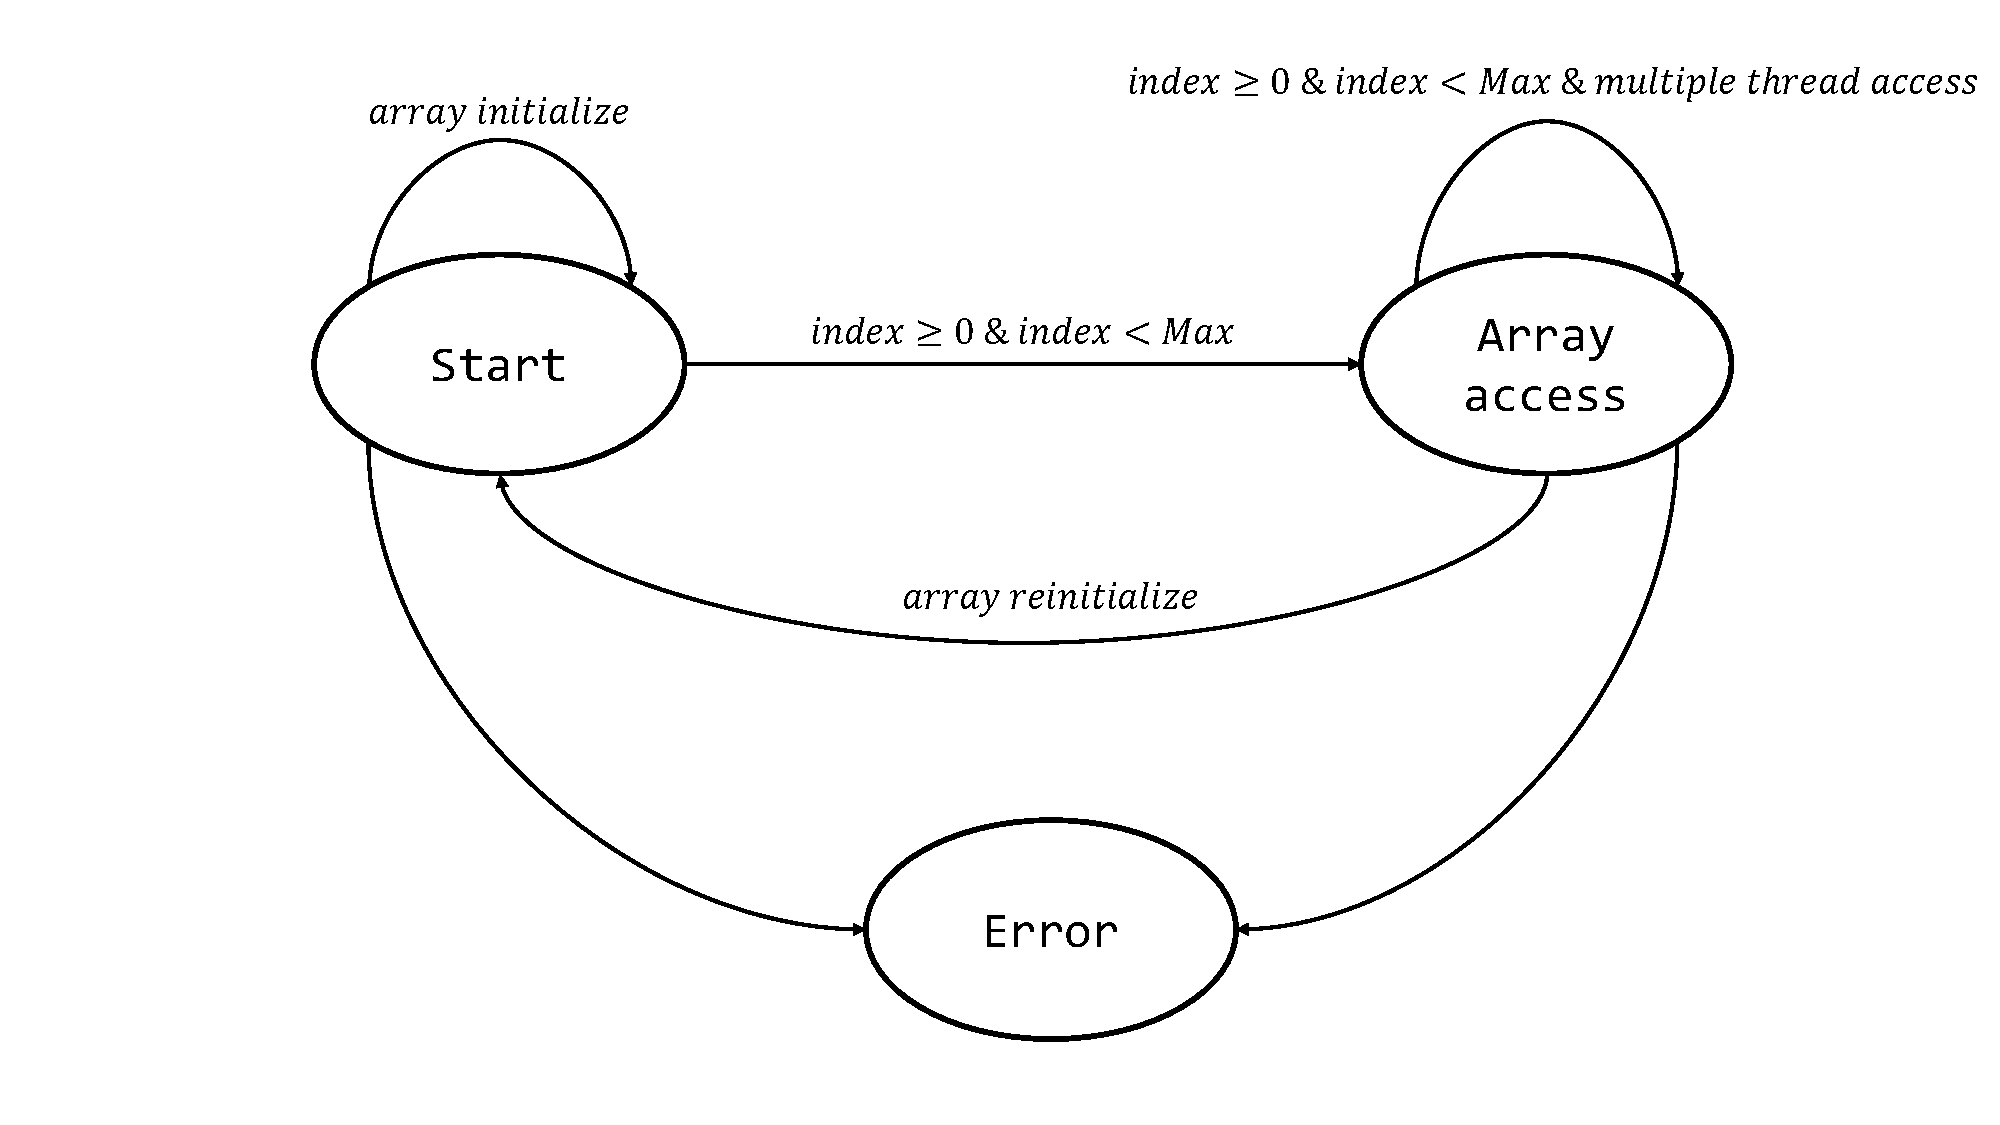
\includegraphics[width=3.2in]{images/ArrayIndex.pdf}
\caption{array index out of bound formulated as FSM}
\label{fig:array}
\end{figure}


We can visualize all runtime exceptions as finite state machine (FSM). When a
program violates such sequence, it throws runtime exception. 
In Figure~\ref{fig:array}, array index out of bound (java.lang.
ArrayIndexOutOfBoundException) exception is described as a FSM. 
Here, a program will be in safe bound as long as the $array\_index \geq 0$ or
$array\_index \leq max\_array\_size - 1$



%%%%%%%%%%%%%%%%%%%%%%%%%%%%%%%%%%%%%%%%%%%%%%%%%

%%%%%%%%%%%%%%%%%%%%%%%%%%%%%%%%%%%%%%%%%%%%%%%%%
%Repairing Strategy:Exception Type
\section{Repairing Strategy: Exception Type}
\label{sec:strgEx}

%marker
\textcolor{red}{\textbf{Please review this section}}\newline

\begin{figure}[t]
\lstset{language=Java, caption=Java code which may throws runtime exceptions,
label=example1}
\begin{lstlisting}[countblanklines=false]
public class TestClass {
    private int[] arr1;
    private int[] arr2;
    private int[] arr3;

    public TestClass(int[] arr1, int[] arr2, int[] arr3) {
	this.arr1 = arr1;
	this.arr2 = arr2;
	this.arr3 = arr3;
    }
    public int[] fun(int a, int b, int c, int d) {
	int temp0 = a + b;
	int temp1 = c * d;
	int temp2 = temp0 - temp1;
	//array index out of bound, negative index
	int temp3 = this.arr1[temp0];
	//array index out of bound, negative index
	int temp4 = this.arr2[temp1];
	//array index out of bound, negative index
	int temp5 = this.arr3[temp3];
	int temp6 = temp4 + temp5;
	int temp7 = temp6 - temp3;
	//array index out of bound, negative index, divide by zero
	this.arr1[temp6] = temp7/(d-a);
	//array index out of bound, negative index, divide by zero
	this.arr2[temp7] = temp7/temp4;
	if(arr2[temp1] ! = arr3[temp7]) return arr1;
	else return null;
    }
}
public class MainClass {
    public void main(String[] a) {
	int[] arr1 = {1,2,3,4};
	int[] arr2 = {1,2,3,4};
	int[] arr3 = {1,2,3,4};
	TestClass TC = new TestClass(arr1, arr2, arr3);
	int[] res = TC.fun(2,4,3,4);
	//Null pointer exception
	System.out.print("Result : "+res[2]);
    }    
}
\end{lstlisting}
\end{figure}

In the Example~\ref{example1}, we have given a piece of \java\ code which shows
multiple lines can throw several runtime exceptions.
In this example we consider three very common runtime exceptions:
NullPointerException, ArrayIndexOutOfBoundExcepltion, NegetiveIndexException,
ArithmeticException (i.e. divide-by-zero). In rest of this section, this
particular example will be used to demonstrate the repairing strategy.

\subsection{Symbolic Analysis}
\label{subsec:symb}


\begin{figure}[t]
\centering
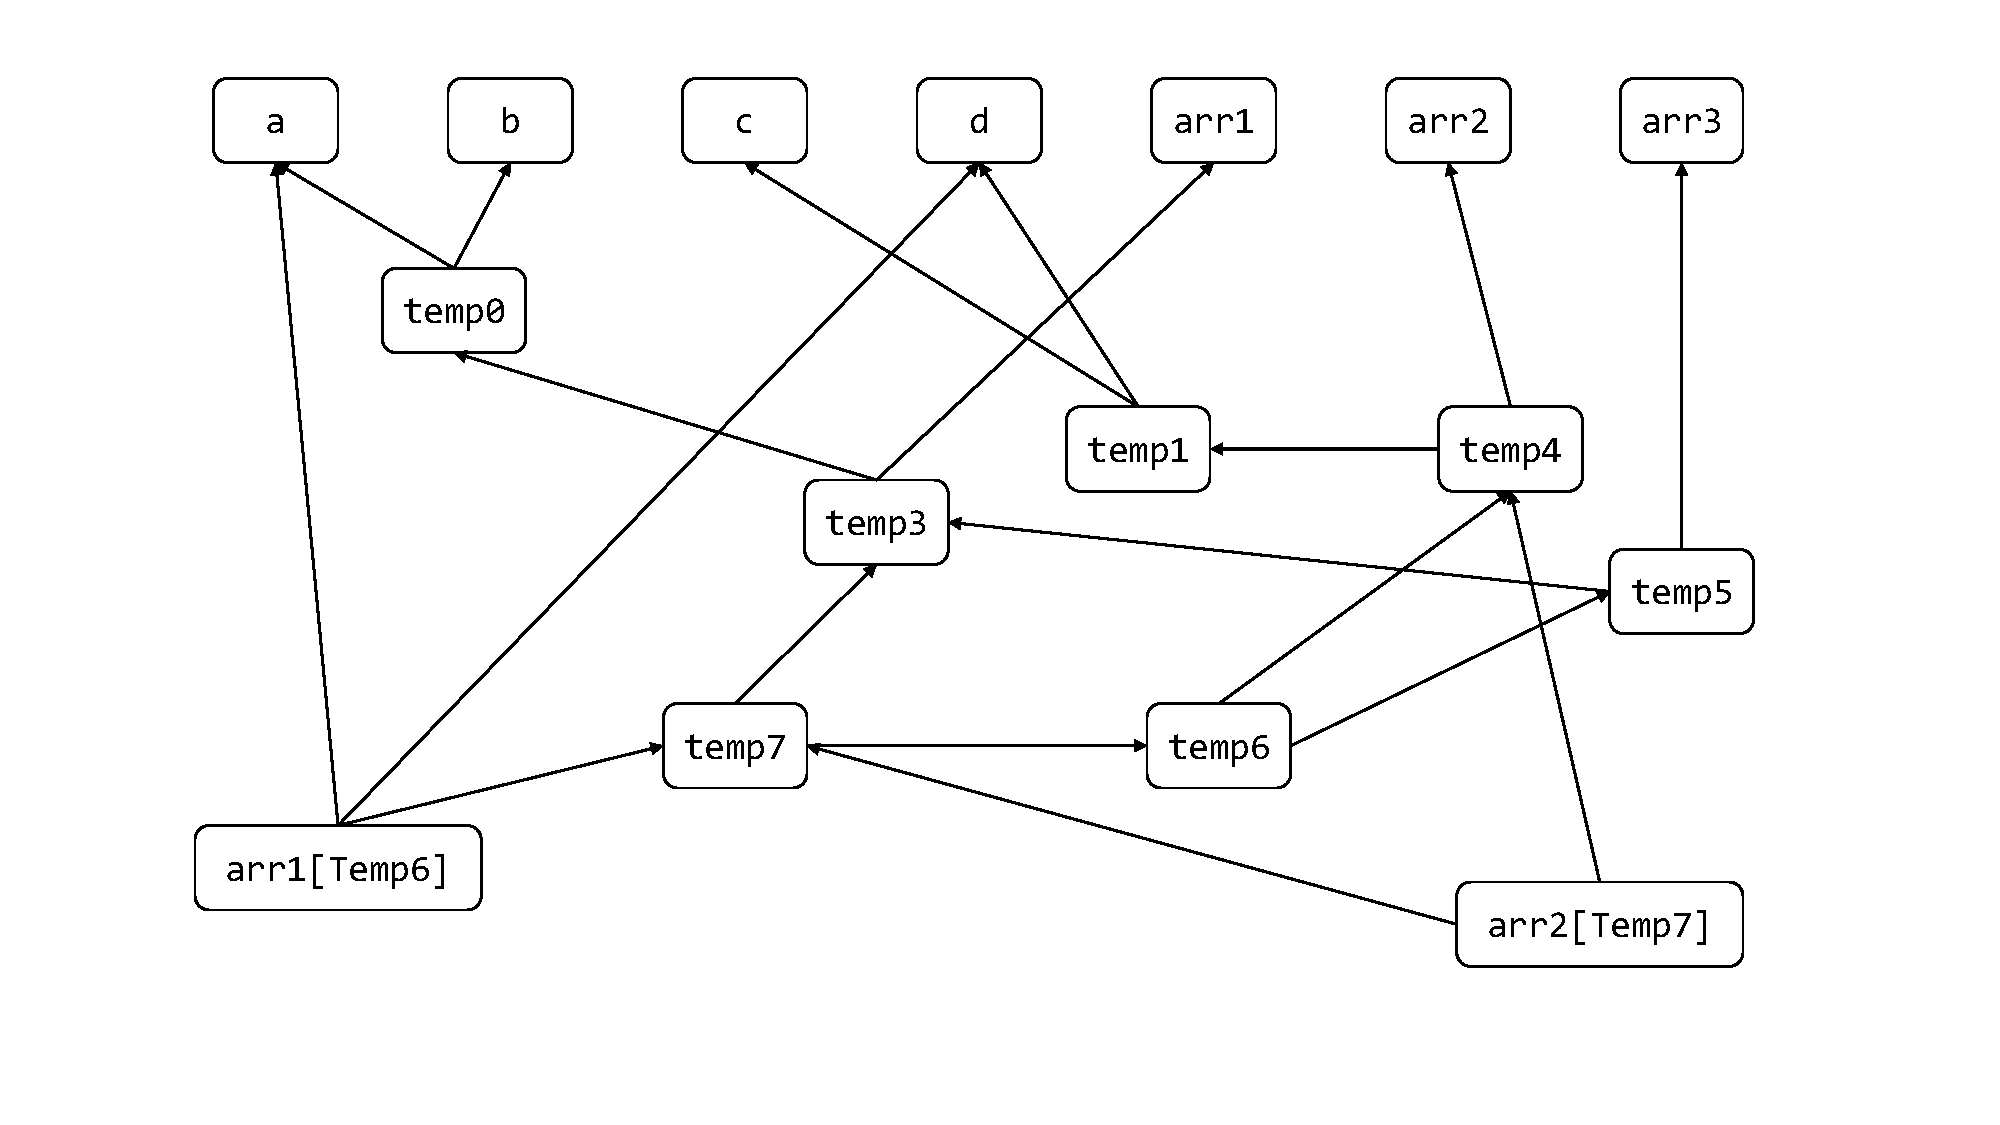
\includegraphics[width=3.3in]{images/depG.pdf}
\caption{Data dependency graph of the variables in Example\ref{example1}}
\label{fig:datadep}
\end{figure}

We have done several  static analysis a priori  over the Java source code to
discover :
\begin{mylist}
\item Critical section of the code which are not eligible for patching. Eg.
banking or any financial transaction which should be crashed in case of
exception as suboptimal solution due to patching will led it to inconsistent
state.
\item Symbolic analysis of the program to discover potential points of failure
and mark them.
\item Build data dependency graph which will be used to generate appropriate
code slice to be used as patch.
In Figure~\ref{fig:datadep}, the data dependency graph of the example
code~\ref{example1} is presented.
\item The symbolic analysis will also reveal which kind of exception is likely
to happened at the time of execution.
This information is necessary at the time of instrumenting the patch as it will
determine the catch block.
	
\end{mylist}

\subsection{Data set for Successful Program Runs}
\label{subsec:progrun}

Here we will store all the traces of successful program runs.
\begin{figure}[t]
\centering
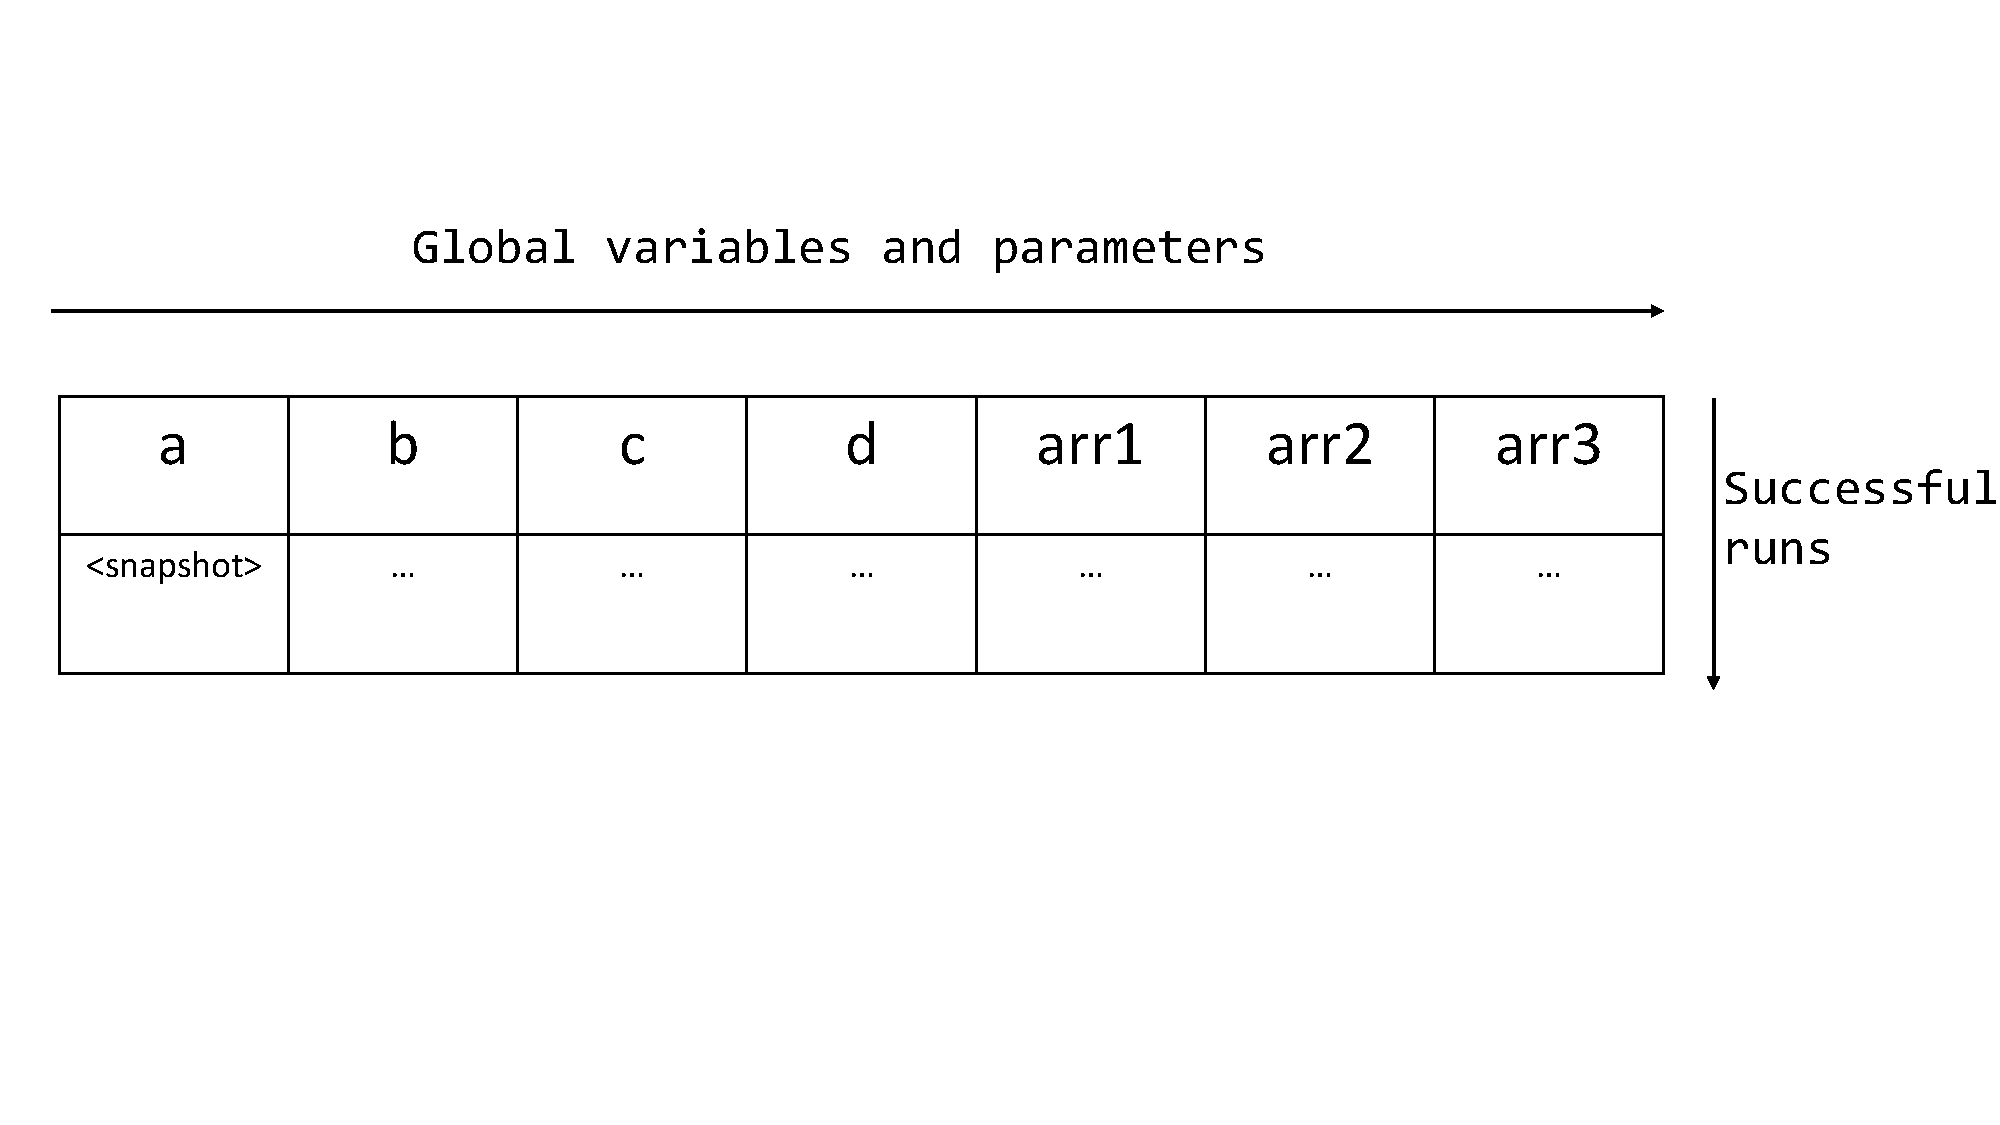
\includegraphics[width=3.0in]{images/succrun.pdf}
\caption{Indexed global variables and method arguments successful runs}
\label{fig:succrun}
\end{figure}

Figure~\ref{fig:succrun} shows such indexed traces of all the global variables
and method arguments.
We store the snapshots of these objects. We won't store local variables as they
can always be regenerated.
As it is required to capture the snapshot of all these variable, we made deep
cone of all of these objects and variables.

% begin{table}[htb]
%\begin{tabular}{|c|c|c|c|c|c|c|}
%\hline
%a & b & c & d & arr1 & arr2 & arr3 \\ \hline
%\ldots & \ldots & \ldots & \ldots &	\ldots & \ldots & \ldots\\ \hline
%\end{tabular}
%\caption{Trace of successful runs}
%	\label{tab:Trace}
%\end{table}


\subsection{Matrices}
\label{subsec:martices}

%marker
\textcolor{red}{\textbf{Please review this section.}}\newline

\subsection{Instrumenting Patching}
\label{subsec:patchinstru}

We have used Soot framework which is a Java byte code manipulator to instrument
patch. 
The patching technique is divided into two phases

\subsubsection{Determine Exception Type} 

At the time of execution, the exception may happened due to some specific values
of some variables. We will catch the exception. Here the type of runtime
exception is $java.lang.ArrayIndexOutOfBound$. This will be used to produce the
try-catch block.
 
\subsubsection{Determine Optimal Code Slice}

The optimal code slice will be determined from the data dependency graph which
was rendered at the time of static analysis mentioned in
Section~\ref{subsec:symb}. In the Listing~\ref{patchingexample1}, the example
code snippet shows such code slice inside the catch block.
As the error occurred at the line $int\ temp5\ =\ this.arr3[temp3];$ the
statements which produces the temp3 and the statement which also involves
$temp3$ or any other variables derived from $temp3$, would be included in the
catch block for re-execution with the valued of the same from the data table of
previous successful runs.

 

\lstset{language=Java, caption=patching code slice based on exception type,
label=patchingexample1}

\begin{figure}[t]
\begin{lstlisting}[countblanklines=false]
public class TestClass {
    private int[] arr1;
    private int[] arr2;
    private int[] arr3;

    public TestClass(int[] arr1, int[] arr2, int[] arr3) {
	this.arr1 = arr1;
	this.arr2 = arr2;
	this.arr3 = arr3;
    }
    public int[] fun(int a, int b, int c, int d) {
	try {
	    int temp0 = a + b;
	    int temp1 = c * d;
	    int temp2 = temp0 - temp1;
	    int temp3 = this.arr1[temp0];
	    int temp4 = this.arr2[temp1];
	    //IndexOutOfBoundException as temp3 = 20
	    int temp5 = this.arr3[temp3];
	    int temp6 = temp4 + temp5;
	    int temp7 = temp6 - temp3;
	    this.arr1[temp6] = temp7/(d-a);
	    this.arr2[temp7] = temp7/temp4;
	} catch(IndexOutOfBoundsException indEx) {
	    int temp0 = a + b;
	    int temp1 = c * d;
	    int temp2 = temp0 - temp1;
	    int temp3 = this.arr1[temp0];
	    //Bellow line is not part of the patch as
	    //temp1 and temp3are not related to temp3
	    //for which the exception occurred.
	    //int temp4 = this.arr2[temp1];
	    int temp5 = this.arr3[temp3];
	}
	if(arr2[temp1] ! = arr3[temp7]) return arr1;
	else return null;
    }
}
public class MainClass {
    public void main(String[] a) {
	int[] arr1 = {20,21,22,23};
	int[] arr2 = {1,2,3,4};
	int[] arr3 = {10,11,12,13};
	TestClass TC = new TestClass(arr1, arr2, arr3);
	int[] res = TC.fun(2,4,3,2);
	System.out.print("Result : " + res[2]);
    }    
}
\end{lstlisting}
\end{figure}

\subsection{Variable Tracking and Monitoring}
\label{subsec:taint}
\textcolor{red}{\textbf{I have added standard taint analysis technique here as
an example. We can change it later}}\newline


Here we used taint analysis technique to tag variables and objects of our
interest to monitor them.
This steps are necessary as the values of the variables used during the
instrumentation may cause further runtime exceptions.
We used bit-vector which is an efficient technique to taint a object/variable.
It requires maintain a single dimension byte array where each bit correspond to
a single object/variable of our interest.
The bit values will be flipped when it is required to taint ($1$) or untaint
($1$) an object/variable.
We will only monitor these entities until all of them flushed from the program
and the entire program reached to a stable state.
%%%%%%%%%%%%%%%%%%%%%%%%%%%%%%%%%%%%%%%%%%%%%%%%%

%%%%%%%%%%%%%%%%%%%%%%%%%%%%%%%%%%%%%%%%%%%%%%%%%
%Repairing Strategy : Constraint Automata
\section{Repairing Strategy : Constraint Automata}
\label{sec:strgCA}

\subsection{General Structure}
\label{subsec:generalCA}

\emph{Constraint automata} is a formalism to describe the behavior and possible
data flow in coordination models. 
Mostly used for model checking. We have used it for the purpose of program
repairing technique. Here we define the finite state automata as follows :

$$(Q, \Sigma, \delta, q_0, F)$$
\begin{itemize}
	\item $Q$: set of state where $|Q| = 2$, \emph{legal state}(init) and
\emph{illegal state} (error).
	\item $\Sigma$: symbols, invariants based on exception type.
	\item $\delta$: transition function. $init \rightarrow init$ is safe
transition and $init \rightarrow error$ is the invariant violation.
	\item $q_0$: starting state, here $q_0 = init$.
	\item $F$: end state, here it same as $q_0$.
\end{itemize}

\begin{figure}[t]
\centering
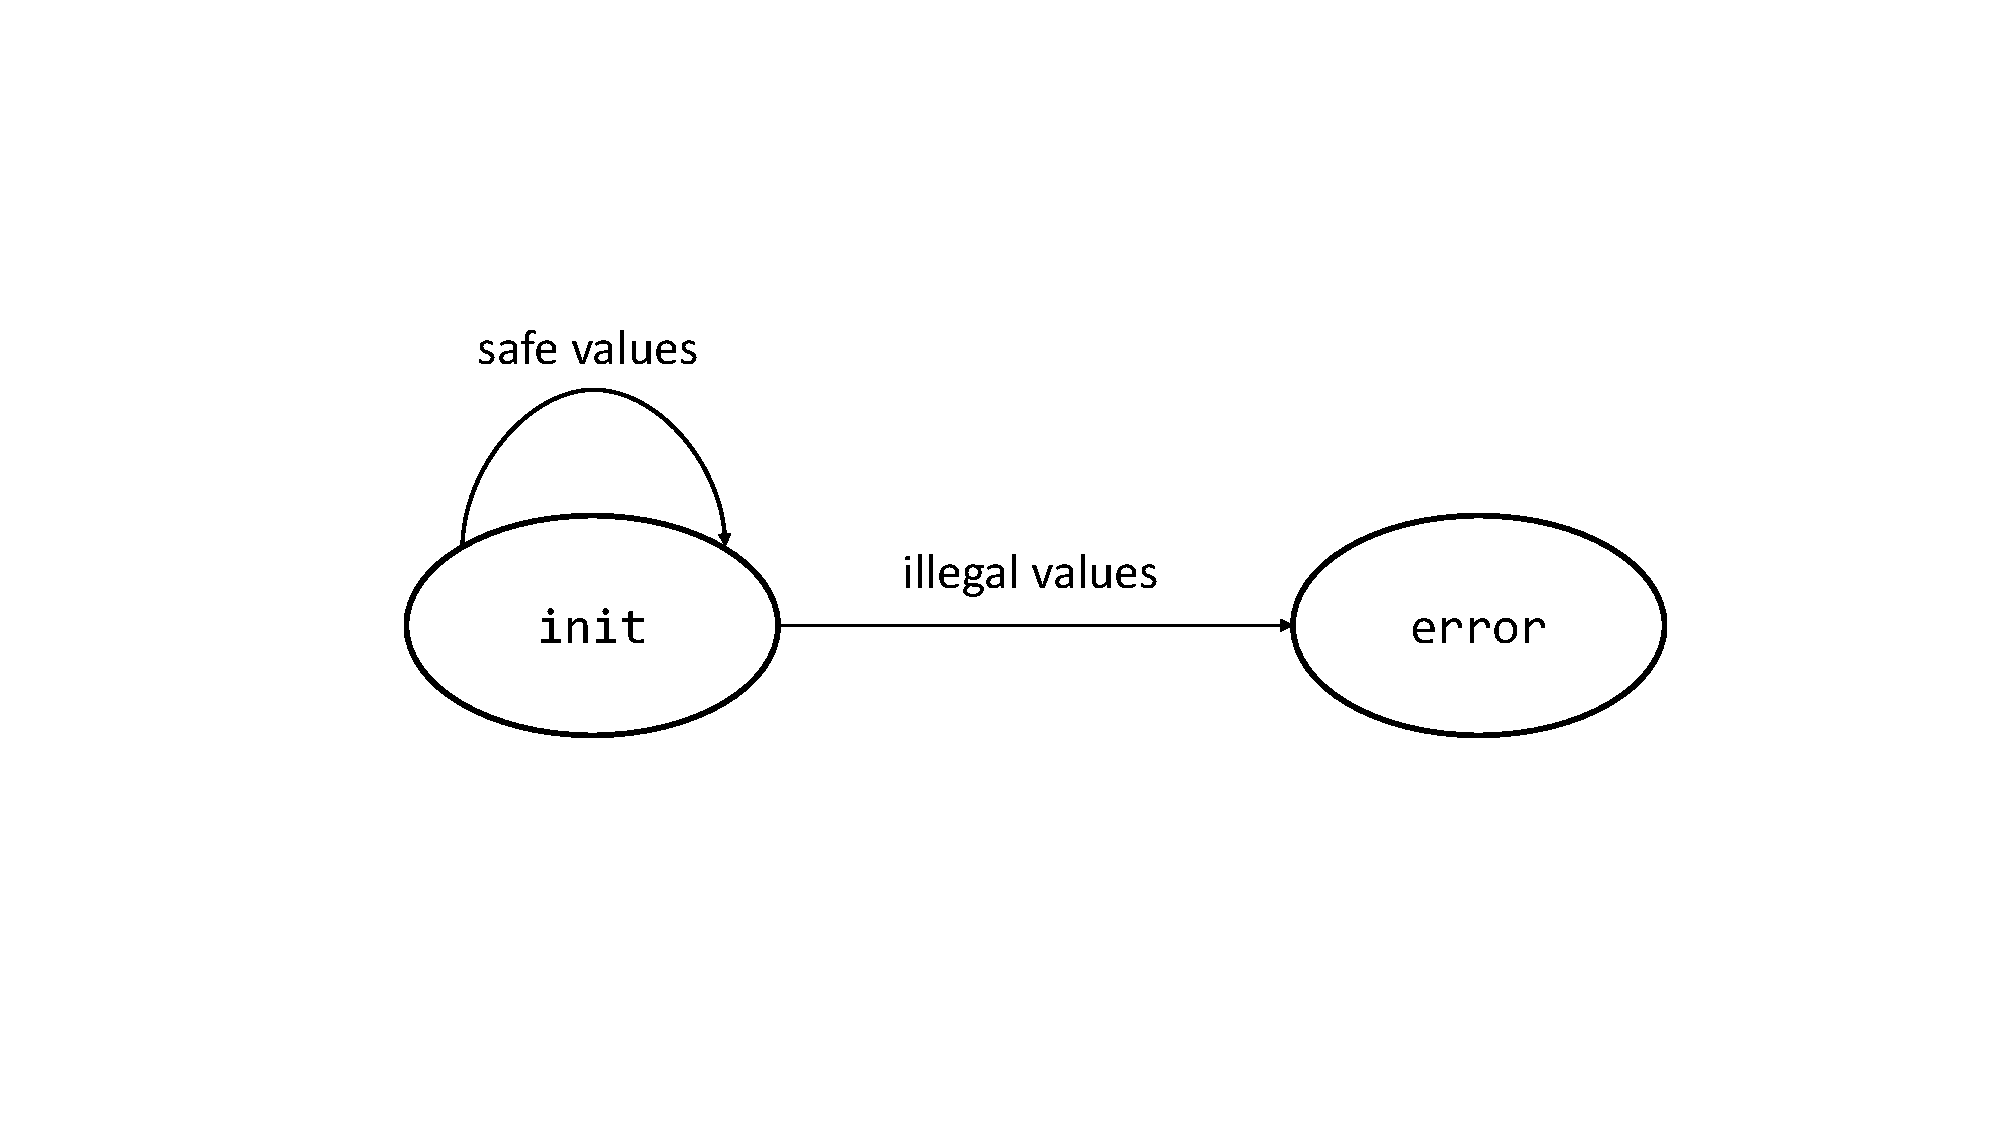
\includegraphics[width=3.2in]{images/automata.pdf}
\caption{Constraint automata general model}
\label{fig:automata}
\end{figure}

According to the Figure~\ref{fig:automata}, the repairing mechanism will only
trigger when we have a transition from 
init state to error state due to invariant violation.

\subsection{Patching Techniques}
\label{subsec:patchCA}

The patching technique is based on the exception type. 

\subsubsection{Array index out of bound exception}

Array index out of bound exception happen when one tries to access the array
with a index which is more than the size of the array or 
less than zero i.e. with some negative value. We did the patching based on these
two scenario. When the index is more than the array size, 
we patch it by assigning $array.length - 1$.

\lstset{language=Java, caption=array index out of bound patching,
label=patchingexample2}
\begin{figure}[t]
\begin{lstlisting}[countblanklines=false]
void foo() {
    int []arr = {1,2,3,4};
    int index = 10;
    int y = 0;
    try {
	//original code
	y = arr[index];
    } catch(IndexOutOfBoundException ex) {
	//patching instrumentation
	if(index > arr.length) y = arr[arr.length - 1];
	else y = a[0];
    }
}
\end{lstlisting}
\end{figure}

\subsubsection{Negative Array Size Exception}

Negative array size exception occurs when one tries to create a array with a
negative size. 
The patching is done based on data flow analysis. Suitable index size is
determined by looking at the successive statement dependent on the array. 
To take a safe bound, we took maximum index size and set as the array size in
the new array statement.


\lstset{language=Java, caption=arr index out of bound patching,
label=patchingexample2}
\begin{figure}[t]
\begin{lstlisting}[countblanklines=false]
void foo() {
    int []arr = {1,2,3,4};
    int index = 10;
    int y = 0;
    try {
	//original code
	y = arr[index];
    } catch(IndexOutOfBoundException ex) {
	//patching instrumentation
	if(index > arr.length) y = arr[arr.length - 1];
	else y = a[0];
    }
}
\end{lstlisting}
\end{figure}

\subsubsection{Arithmetic Exception : Division-by-zero Exception}

Division by zero causes arithmetic exception. There are two different cases
which were considered here. 
\begin{itemize}
 \item \textbf{Case I :} The denominator is going to the taint sink but
the left hand side is not going to any taint sink. Here we will not
manipulate the denominator as we are not manipulating any variable which are
going to any taint sink.
 \item \textbf{Case II :} The denominator and the left hand side, both are not
going to any taint sink. So they are safe to patch.
\end{itemize}

\lstset{language=Java, caption=arithmetic exception : division-by-zero patching,
label=patchingexample2}
\begin{figure}[t]
\begin{lstlisting}[countblanklines=false]
void foo() {
    int a = 10;
    int b = 0;
    int y;
    try {
	//original code
	y = a/b;
    } catch(ArithmeticException ex) {
	//patching instrumentation
	//case I
	if(taintSink(b)) y = 0;
	//case II
	else {
	    b = 1;
	    y = a/b;
	}
    }
}
\end{lstlisting}
\end{figure}

\subsubsection{Null Pointer Exception}

Null pointer exception in Java is the most common runtime exception
encountered. 
Thrown when an application attempts to use null in a case where an object is
required. There exists various scenarios where null pointer exception can
happen. These different scenario requires different patching techniques. Bellow
we enlist all cases and corresponding patching techniques.


\begin{itemize}
  \item \textbf{Case I} Calling the instance method of a null object. \newline
  \textbf{Patch :} This is patched by calling the constructor. In case there
  exists more than one constructor then we need to find most appropriate
  constructor. This is done by using data flow analysis in the successive
  statement to see which fields/methods been accessed and according to that
  most suitable constructor should be picked up, this will ensure safest way to
  deal with the later method calls/field accesses.
  
  \lstset{language=Java, caption=appropriate constructor,
label=patchingexample2}

\begin{figure}[t]
\begin{lstlisting}[countblanklines=false]
class MyClass {
    Integer field1;
    String field2;
    Double field3;

    public MyClass(){
	this.field1 = 1;
	this.field2 = null;
	this.field3 = null;
    }
    public MyClass(Integer field1, String field2) {
	this.field1 = field1;
	this.field2 = field2;
	this.field3 = null;
    }
    public MyClass(Integer field1, String field2, Double field3) {
	this.field1 = field1;
	this.field2 = field2;
	this.field3 = field3;
    }
    public Double getfield3() {
	return this.field3;
    }
}

class main {
    Myclass mclass = null;
    Double a = null;
    try {
	//original code
	a = mclass.getfiled3() + 5.0;
    } catch(NullPointerException ex) {
	//instrumentation
	//choose appropriate constructor
	mlass = new MyClass(1, "a", 1.0);
	a = mclass.getfiled3();
    }
}
\end{lstlisting}
\end{figure}

  \item 
  
  \item \textbf{Case II} Possible Accessing or modifying the field of a null
  object.\newline
  \textbf{Patch :} The patch is same as the previous one.
  
  \item \textbf{Case III} Taking the length of null as if it were an
  array.\newline
  \textbf{Patch :}The patch for this situation is very much similar to the
  negative array size exception. Here we will do a data-flow analysis to see all
  the successive statements where the array object has been used (read or
  write). For safety we will take the maximum index from those statements and
  reinitialize the array object with the size.
    
  \lstset{language=Java, caption=array null pointer exception,
  label=patchingexample2}

\begin{figure}[t]
\begin{lstlisting}
int[] bar(int a) {
    int []arr = new int[a];
    int []b = (a > 10) ? arr:null;
    return b;
}
void foo() {
    int[] arr;
    int []arr = bar(5);
    try {
	//access or modify any field of arr
	//this will throw a null pointer exception
    } catch {
	//instrumented code
	int ARRAY_SIZE = 11;
	int []arr = new int[ARRAY_SIZE];
	//access or modify any field of arr
    }
}
\end{lstlisting}
\end{figure}

  \item \textbf{Case IV} Accessing or modifying the slots of null as if it were
  an array.
 \textbf{Patch :} The patching mechanism is exactly same as before.
 
  \item \textbf{Case V} Throwing null as if it were a Throwable value.
\end{itemize}
%%%%%%%%%%%%%%%%%%%%%%%%%%%%%%%%%%%%%%%%%%%%%%%%%

%%%%%%%%%%%%%%%%%%%%%%%%%%%%%%%%%%%%%%%%%%%%%%%%%
%Design of the System
\section{Design of the System}
\label{sec:SystemDesign}


%later convert this pdf
\begin{figure}[t]
\centering
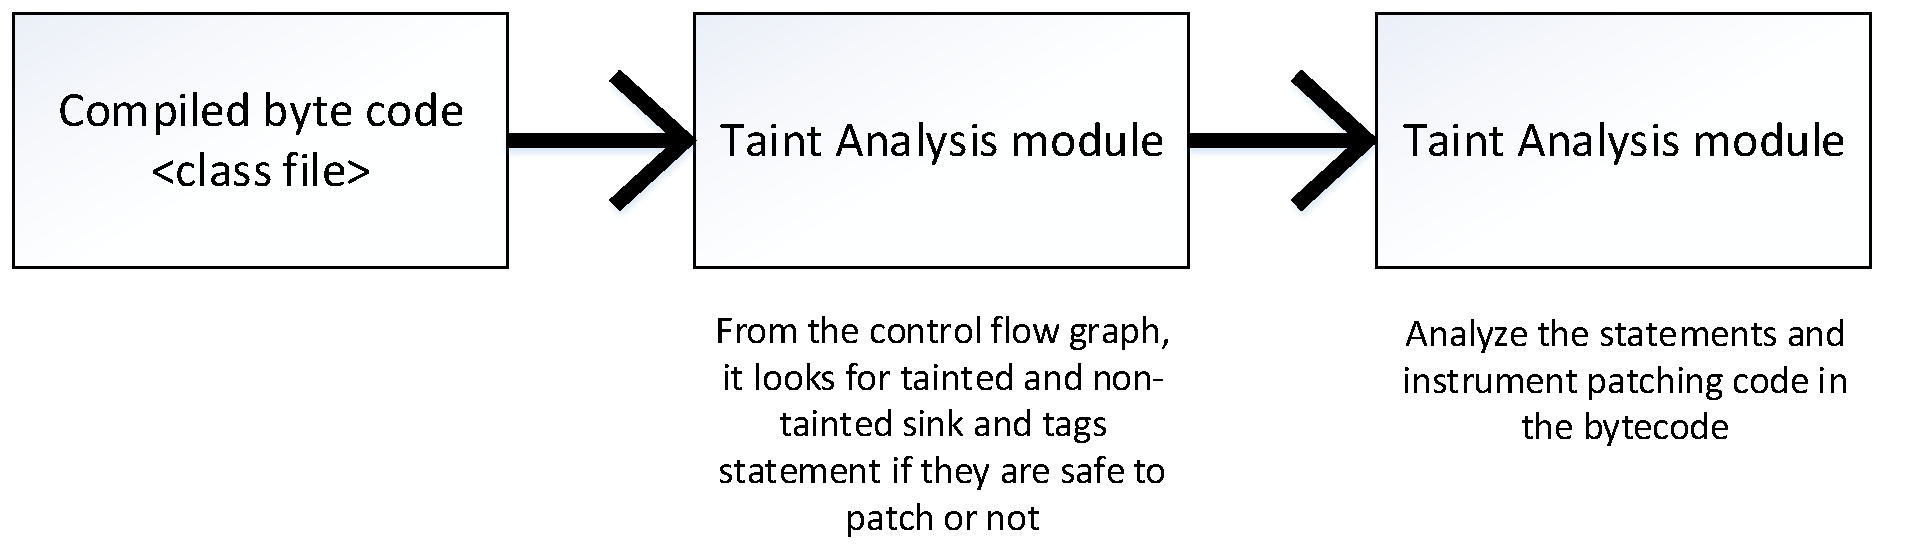
\includegraphics[width=3.2in]{images/OverallDesign.png}
\caption{Overall Design}
\label{fig:overallDesign}
\end{figure}


% \begin{figure}[!htb]
% \centering
% 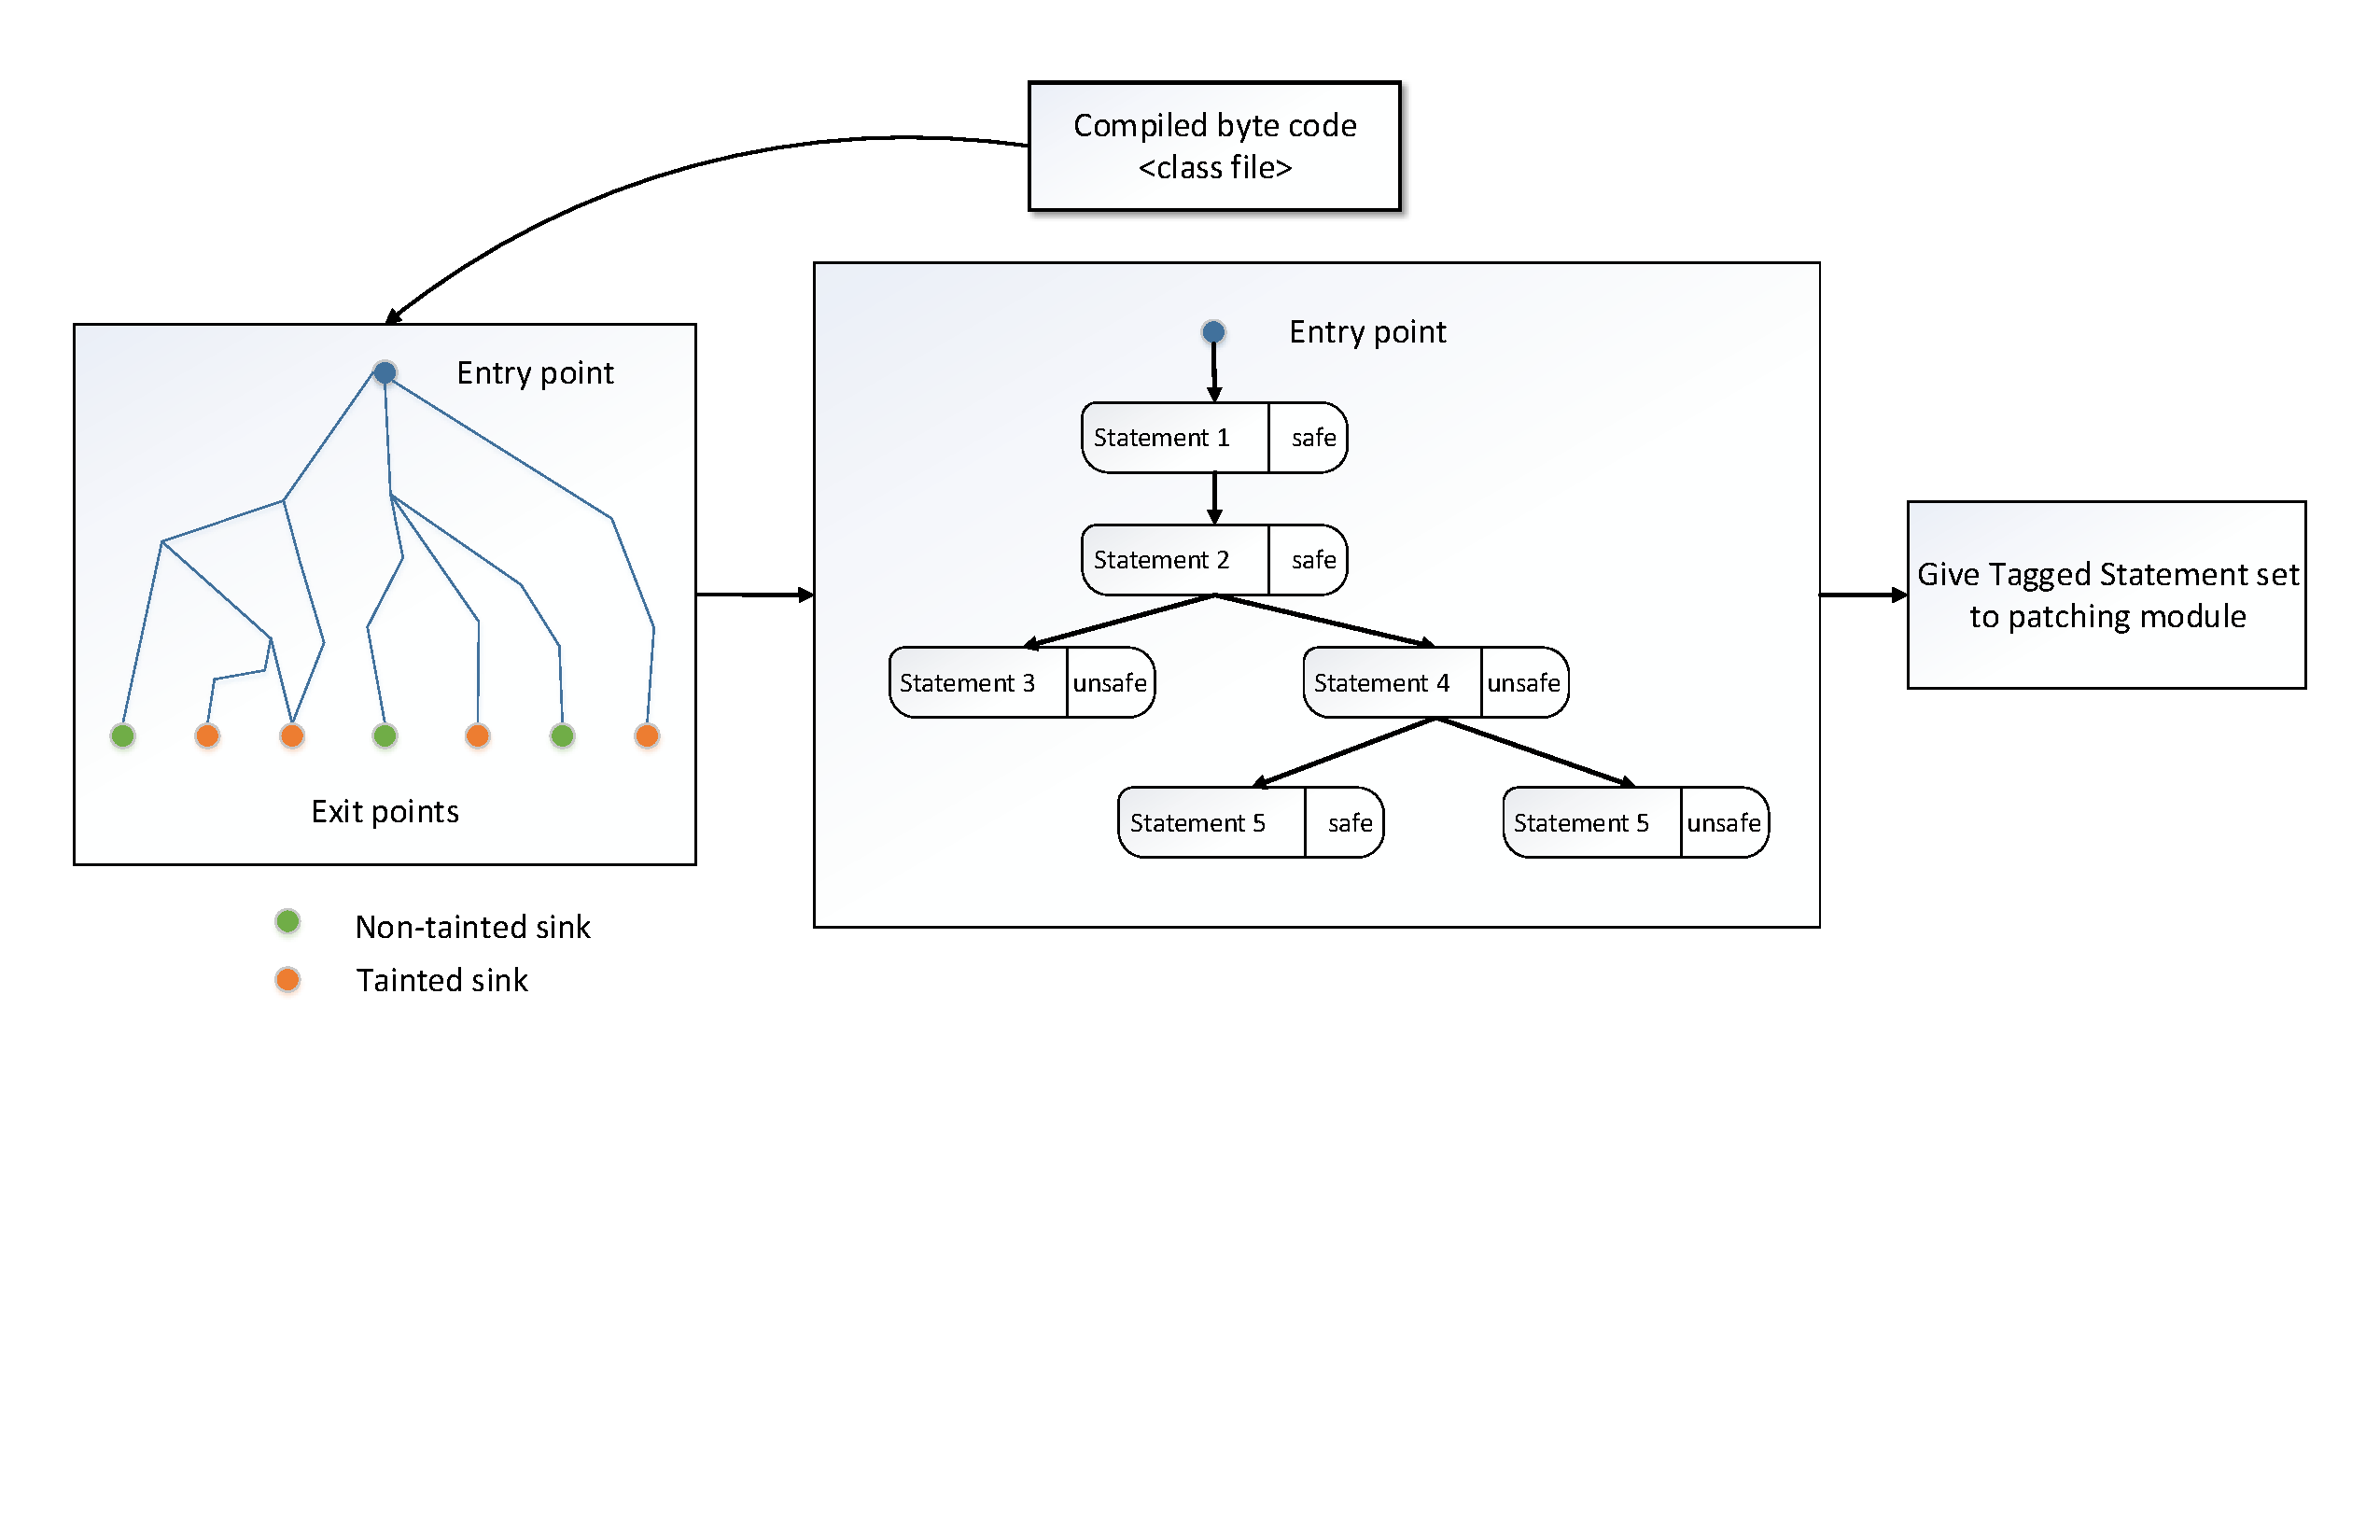
\includegraphics[width=3.5in]{images/TaintModule.pdf}
% \caption{Overall Design}
% \label{fig:TaintModule}
% \end{figure}
% 
% \begin{figure*
%   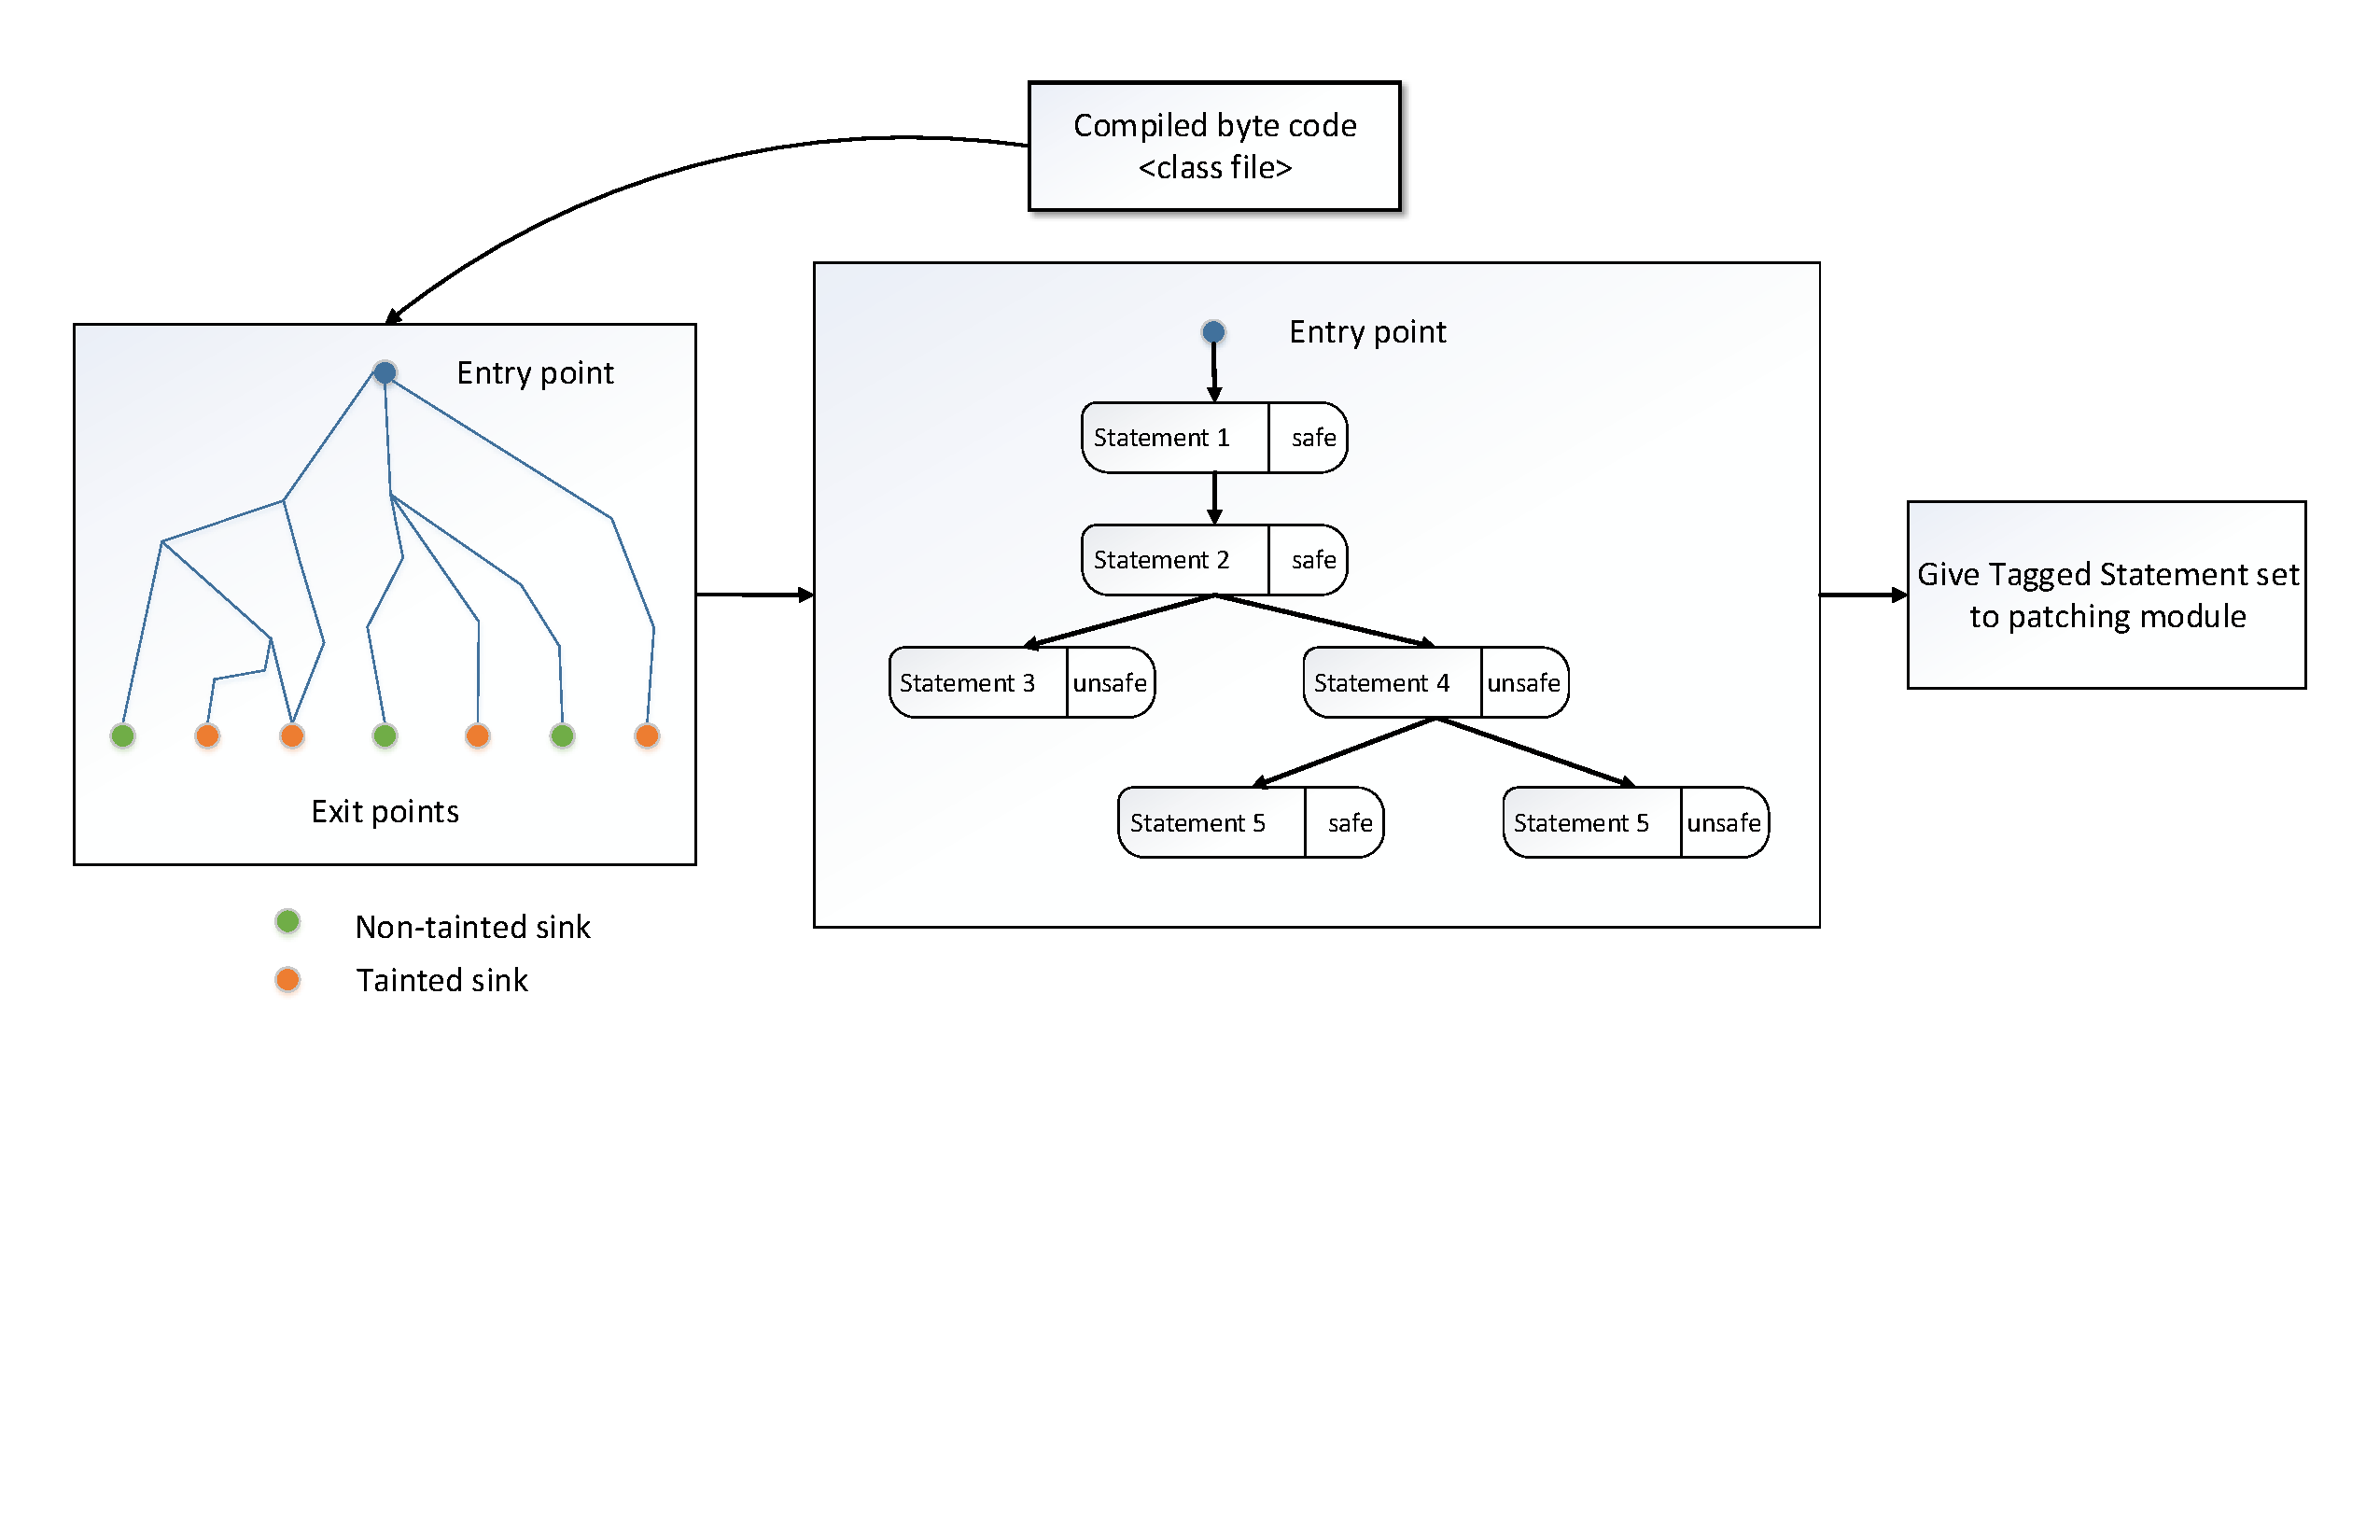
\includegraphics[width=\textwidth,height=5cm]{images/TaintModule.pdf}
%   \caption{Design of the Taint Module}
% \end{figure*}

%later covert this to pdf
\begin{figure*}[t]
\centering
  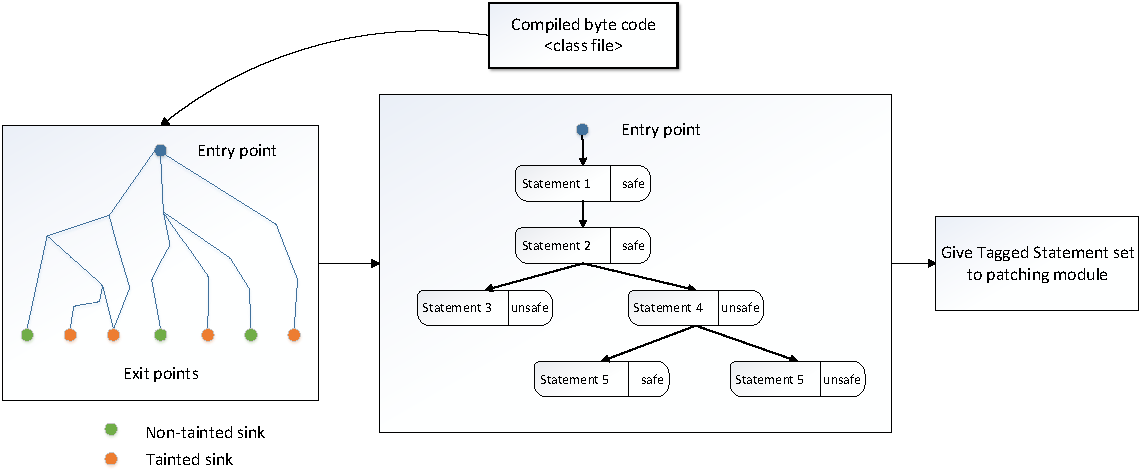
\includegraphics[width= 7.0in]{images/TaintModule.png}
  \caption{Design of the Taint Module}
  \label{fig:TaintModule}
\end{figure*}


The overall design of the repairing framework is illustrated in
Figure~\ref{fig:overallDesign}. The framework consists of two basic modules.


\subsection{Taint analysis Module}
\label{subsec:TaintModule}

The main purpose of the taint analysis module is to classify which of the
statements are safe to patch or not. Based on the analysis result in this
module, the tagged statement will be passed to the repairing module.


We have specify the list of source, sink and derivation methods in a
configuration file before the analysis. The source methods includes methods
which
take input from user from console or web application forms like text box. The
sink methods are sensitive data storage which are unsafe to manipulate such as
database, console print or methods to send a text file to printer etc. The
overview of the taint analysis module is illustrated in the
Figure~\ref{fig:TaintModule}.  The input for the module is the compiled byte
code intended to be repaired. Here we have generated a control flow graph (CFG)
from the class file to get all the possible program paths. Here a point to be
noted that any modification along the path going to the tainted sink is unsafe
to patch.


\subsubsection{Tainting Rules}
\label{subsubsec:TaintingRule}
\textcolor{red}{\textbf{Needs Revision}}\newline

\begin{table}[t]
\centering
\small
\begin{tabular}{l|l}
\multicolumn{1}{c|}{\textbf{\java\ Class}} & \multicolumn{1}{c}{\textbf{Source
Method}}\\
% \scalebox{0.86}
% {
\hline
\code{java.io.InputStream} & \code{read()}\\
\code{java.io.BufferedReader} & \code{readLine()}\\
\code{java.net.URL} & \code{openConnection()}\\
\code{org.apache.http.HttpResponse} & \code{getEntity()}\\
\code{org.apache.http.util.EntityUtils} & \code{toString()}\\
\code{org.apache.http.util.EntityUtils} & \code{toByteArray()}\\
\code{org.apache.http.util.EntityUtils} & \code{getContentCharSet()}\\
\code{javax.servlet.http.HttpServletRequest} & \code{getParameter()}\\
\code{javax.servlet.ServletRequest} & \code{getParameter()}\\
\code{java.Util.Scanner} & \code{next()}\\
\end{tabular}
\caption{Common \java\ library taint source functions}
\label{tab:TaintSources}
% }
\end{table}



\begin{table}[t]
\centering
\small
\begin{tabular}{l|l}
\multicolumn{1}{c|}{\textbf{\java\ Class}} & \multicolumn{1}{c}{\textbf{Sink
Method}}\\
% \scalebox{0.86}
% {
\hline
\code{java.io.PrintStream} & \code{printf()}\\
\code{java.io.OutputStream} & \code{write()}\\
\code{java.io.FileOutputStream} & \code{write()}\\
\code{java.io.Writer} & \code{write()}\\
\code{java.net.Socket} & \code{connect()}\\
%org.apache.http.impl.client.DefaultHttpClient & execute\\ \hline
\end{tabular}
% }
\caption{Common \java\ library taint sink functions}
\label{tab:TaintSinks}
\end{table}


We have used extended InFlow framework for the taint analysis module. The steps
are

\begin{mylist}
  \item We defined list of source and sink taint methods listed in
  Table~\ref{tab:TaintSources} and \ref{tab:TaintSinks}. We are only tainting
  the variables which are coming from the listed taint source methods.
  
  \item We have also listed all taint propagation methods. The assignment ($=$)
  is the basic taint propagator. But there are other methods like \code{append}
  in \code{java.lang.StringBuffer} and \code{java.lang.StringBuilder} which are
  taint propagator.

  \item All the variable which are referred to tainted variables/ objects or
  output of taint propagator over tainted variable/objects are also considered
  as tainted.

  \item For all the program patch we see if such tainted variables are reaching
  the tainted sink or not. If they are reaching to some tainted sink then all
  the statements along that particular program path to which the tainted
  variables are assigned are marked as unsafe otherwise safe.
\end{mylist}


\subsection{Repairing Module}
\label{subsec:RepairingModule}

%later covert this to pdf
\begin{figure}[t]
\centering
  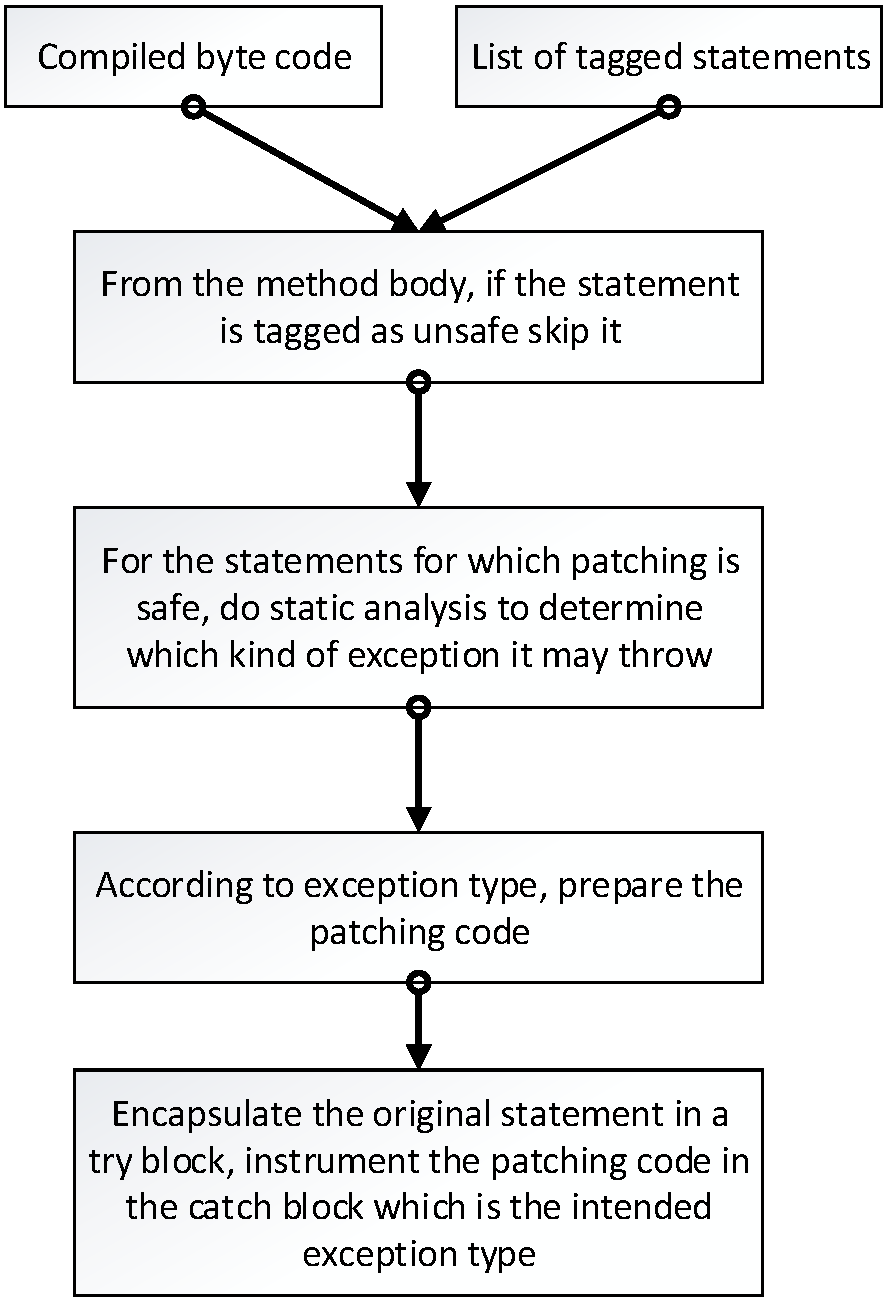
\includegraphics[scale= .5]{images/PatchModule.png}
  \caption{Design of the Patching Module}
  \label{fig:PatchModule}
\end{figure}

The repairing module is consisted of three phases. All these three phases
requires three sequential passes over the input bytecodes to produce the final
patched result.


\subsubsection{Method Shilding}
\label{MethodShilding}


When we are shielding a method, we also looked to the calling context of that
particular method. The method can be called from a path which leads to some
tainted sink and it can also be called from such path which does not contain
any taint sink. In such cases, we have taken special care about the callee. The
path to the tainted sink should not call a patched method as it can influence
data which are leaving the system. So, we also maintained two different version
of
the method and instrument the calling site so that appropriate method is called.

\lstset{language=java, caption = Same method calling in different scenario,
label=callingContext}
\begin{figure}[t]
\begin{lstlisting}[countblanklines=false]
int bar(int a, int b) {
    return a/b;
}
void foo() {
    int a = 10, b = 0, c = 15;
    int out = bar(a, b);
    TaintSink(out);
    int out1 = bar(c, b);
    NonTaintSink(out1);
}
\end{lstlisting}
\end{figure}

\lstset{language=java, caption = Method name modification for different calling
context, label=callingContextPatch}
\begin{figure}[t]
\begin{lstlisting}[countblanklines=false]
int bar(int a, int b) {
    return a/b;
}
int bar_untainted_fa844d57(int a, int b) {
    int out;
    try {
	out = a/b;
    } catch(ArithmeticException ex) {
	b = 1;
	out = a/b;
    }
    return out;
}
void foo() {
    int a = 10, b = 0, c = 15;

    // no modification in the call where the result can go to a tainted sink
    // method
    int out = bar(a, b);
    TaintSink(out);

    // Modify the method call to the shielded method as the result is not going
    // to any tainted sink method
    int out1 = bar_untainted_fa844d57(c, b);
    NonTaintSink(out1);
}
\end{lstlisting}
\end{figure}

In the Listing~\ref{callingContext} and \ref{callingContextPatch} we have
defined an example code snippet of the original code and the patched code where
we have renamed the method \emph{bar} to \emph{bar\_untainted\_fa844d57}
before instrumenting any patching code in it. The variable \emph{out} goes to a
tainted sink while \emph{out1} does not. So the we have done modification in the
line where \emph{out1} is defined. As \emph{out} is going to a tainted sink
method, we did not do any modification to it.



% \begin{enumerate}
%   \item \textbf{Taint analysis module :}
%   \item \textbf{Repairing Module : }
% \end{enumerate}

%%%%%%%%%%%%%%%%%%%%%%%%%%%%%%%%%%%%%%%%%%%%%%%%%

%%%%%%%%%%%%%%%%%%%%%%%%%%%%%%%%%%%%%%%%%%%%%%%%%
%Benchmark Results

\section{Benchmark Results}
\label{sec:bench}
%%%%%%%%%%%%%%%%%%%%%%%%%%%%%%%%%%%%%%%%%%%%%%%%%

%%%%%%%%%%%%%%%%%%%%%%%%%%%%%%%%%%%%%%%%%%%%%%%%%
%Related Work


\section{Related Work}
\label{sec:relatedWorks}

\subsection{Recent Works on Data Structure Repairing}
\label{subsec:RecWorksDataStructure}

Automated data-structure repairing techniques are there in the literature for a
while. In the papers~\cite{conf/oopsla/DemskyR03, Demsky03automaticdata,
conf/icse/DemskyR05, conf/issre/DemskyR03, conf/issta/DemskyEGMPR06} the authors
mostly concentrated on specific data-structures like \emph{FAT-32}, \emph{ext2},
\emph{CTAS} (a set of air-traffic control tools developed at the NASA Ames
research center) and repairing them. The authors represented a specification
language by which they able to see consistency property these data-structure.
Given the specification, they able to detect the inconsistency of these
data-structures and repair them.
The repairing strategy involves detecting the consistency constraints for the
particular data structure, for the violation, they replace the error condition
with correct proposition. In the paper~\cite{conf/icse/DemskyR05}, the authors
Brian Demsky and Martin C. Rinard proposed repair strategy by goal-directed
reasoning. This involves translating the data-structure to a abstract model by a
set of model definition rules. The actual repair involves model reconstruction
and statically mapped it to a data structure update. In their
paper~\cite{conf/oopsla/2007} authors Bassem Elkarablieh, Sarfraz Khurshid, Duy
Vu, Kathryn S. McKinley proposed the idea to statically analyze the data
structure to access the information like recurrent fields and local fields. They
used their technique to some well known data structures like singly linked list,
sorted list, doubly liked list, N-ary tree, AVL tree, binary search tree,
disjoint set, red-black tree, Fibonacci heap etc.

\subsection{Works on Software Patching}
\label{subsec:RecWorksSoftPatch}

In their paper~\cite{conf/sosp/PerkinsKLABCPSSSWZER09}, authors Jeff H.
Perkins, Sunghun Kim, Samuel Larsen, Saman P. Amarasinghe, Jonathan Bachrach and
Michael Carbin, Carlos Pacheco, Frank Sherwood, Stelios Sidiroglou, Greg
Sullivan, Weng-Fai Wong,Yoav Zibin, Michael D. Ernst and Martin C. Rinard
presented their \emph{Clear view} system which works on windows x86 binaries
without requiring any source code. They used invariants analysis for which they
used Daikon~\cite{journals/scp/ErnstPGMPTX07}. They mostly patched security
vulnerabilities by some candidate repair patches.

Fan Lon et al in their paper~\cite{conf/pldi/LongSR14} presented their new
system \emph{RCV} which recovers applications from divide-by-zero and
null-deference error. Their tool replaces \emph{SIGFPE} and \emph{SIGSEGV}
signal handler with its own handler. The approach simply works by assigning zero
at the time of divide-by-zero error, read zero and ignores write at the time of
null-deference error. Their implementation was on $x86$ and $x86-64$ binaries
and they also implemented a dynamic taint analysis to see the effect of
their
patching until the program stabilizes which they called as \emph{error
shepherding}.

\subsection{Genetic Programming, Evolutionary Computation}
\label{subsec:RecWorksGeneric}

Reserch works on program repair based on genetic programming and evolutionary
computation can be found in the paper of Stephanie Forrest, ThanhVu Nguyen,
Westley Weimer and Claire Le Goues~\cite{conf/gecco/2009g} and Westley Weimer,
Stephanie Forrest, Claire Le Goues, ThanhVu
Nguyen~\cite{journals/cacm/WeimerFGN10} respectively. In the papers, the authors
used genetic programming to generate and evaluate test cases. They used their
technique on the well known Microsoft Zune media player bug causing the
application to freeze up.



%%%%%%%%%%%%%%%%%%%%%%%%%%%%%%%%%%%%%%%%%%%%%%%%%

%%%%%%%%%%%%%%%%%%%%%%%%%%%%%%%%%%%%%%%%%%%%%%%%%
%Conclusion and Future Works
\section{Conclusion and Future Work}
\label{sec:conc}

Running programs may crash unexpectedly due to vulnerabilities in the code and
malformed data.
The cost associated with such crashes can be vary with the criticality of the
applications. Therefore, it is hardly a surprise that automatic program
repairing has been an actively researched area over the past decade.
In this work, we have presented a novel program repairing technique, and a tool
\tool\ based on it which employs hybrid program analysis to protect a running
program from failures originating from string-handling errors leading to a
program crash.
Our choice of \java\ \code{String} APIs is driven mainly by the popular usage of
string objects and bugs associated with them.
By focusing on a specific data type, and taking the program context into
account, \tool\ can develop patches that are precise and  semantically close to
the ones developed by the developers.
Hence, when the patches are activated, the program exhibits a behavior which is
close to the intended program behavior.

%this part is now in discussion section
Our study shows that \tool\ can handle programs that are real, and can produce
patches efficiently. Motivated by the results of our study as well as by the
research conducted by other researchers, we intend to extend \tool\ in the
future by adding support for other \java\ APIs and also by adding more
intelligence to the process of patch generation.

%%%%%%%%%%%%%%%%%%%%%%%%%%%%%%%%%%%%%%%%%%%%%%%%%
%\appendix
%\section{Appendix Title}

\acks


% We recommend abbrvnat bibliography style.

\bibliographystyle{abbrvnat}

% The bibliography should be embedded for final submission.
\bibliography{Aritrabib}


%\begin{thebibliography}{}
%\softraggedright


%\end{thebibliography}

\end{document}

%                       Revision History
%                       -------- -------
%  Date         Person  Ver.    Change
%  ----         ------  ----    ------

%  2013.06.29   TU      0.1--4  comments on permission/copyright notices

